%\documentclass[a4paper,11pt]{book}
\documentclass[12pt,letterpaper,twoside,openright]{book}

\def\magyarOptions{defaults=hu-min}
\usepackage[magyar]{babel}
\usepackage{t1enc}% for automatic hyphenation of accented chars
\usepackage[utf8]{inputenc}% for typing chars
\usepackage[T1]{fontenc}
\usepackage{amssymb,amsmath}
\usepackage{indentfirst}
\usepackage{graphicx}
%\usepackage{subfig}
\usepackage[font=it]{caption}
\usepackage{color}
\usepackage{caption}
\usepackage{subcaption}
\usepackage{amsfonts}
\usepackage{siunitx}
\usepackage{ulem}
\usepackage{bm}
\linespread{1.5}
\usepackage{anysize}
\marginsize{3cm}{3cm}{2cm}{2cm}

\makeatletter
\def\footnoterule{\kern-3\p@
  \hrule \@width 2in \kern 2.6\p@} % the \hrule is .4pt high
\makeatother

\frenchspacing
\sloppy 

\usepackage{fancyhdr}
\pagestyle{empty}

\pagestyle{fancy}
\lhead{}
\chead{}
\rhead{}
\fancyfoot{}
\lfoot{}
\cfoot{}
\rfoot{}
\usepackage{fancyhdr}
\renewcommand{\headrulewidth}{0pt}
\makeatletter
\newcommand*{\rom}[1]{\expandafter\@slowromancap\romannumeral #1@}
\makeatother
%\numberwithin{equation}{section}

\usepackage{times}
\usepackage{t1enc}
\usepackage{graphicx}
\usepackage{multirow}
\author{Horváth Bendegúz}
\title{Photo Z}
\date{}

\begin{document}

\begin{titlepage}
\thispagestyle{empty}
\begin{center}
{\color{white}Horváth Bendegúz}
\vspace{150 pt}
\hrule height 1pt
\vskip 0.3 cm
\begin{LARGE}
Gépi tanulási módszerek a fotometrikus vöröseltolódás-becslésben\end{LARGE}
\vskip 0.3 cm
\hrule height 1pt

\vskip 0.3 cm

\begin{small}
Fizika BSc szakdolgozat
\end{small}

\vskip 2 cm

\begin{Large}
Horváth Bendegúz
\end{Large}

\vskip 0.2 cm

\begin{small}
az ELTE TTK Fizika BSc hallgatója
\end{small}

\vskip 3 cm

\begin{table}[!h]
\begin{center}
\begin{tabular}{lr}

\textbf{Témavezető:}& \begin{large}Dr. Csabai István\end{large} egyetemi tanár, Komplex Rendszerek Fizikája Tanszék
\end{tabular}
\end{center}
\end{table}

\vspace{\stretch{1}}
Budapest, 2018 május

\end{center}
\end{titlepage}
\newpage

\chapter*{\centering \begin{normalsize}Kivonat\end{normalsize}}
\thispagestyle{empty}
\begin{quotation}
\noindent % abstract text
Ide kell megírnom a kivonatot.
\end{quotation}
\clearpage



\tableofcontents
%\listoffigures


\pagestyle{fancy}
\lhead[\bfseries \leftmark]{\bfseries \rightmark}
\lhead[\bfseries \nouppercase{\rightmark}]{\bfseries \nouppercase{\leftmark}}
\chead{}
\rhead{\thepage}
\fancyfoot{}
\lfoot{}
\cfoot{}
\rfoot{}
\renewcommand{\headrulewidth}{0.4pt}
\renewcommand{\footrulewidth}{0pt}
\renewcommand{\sectionmark}[1]{\markright{\thesection.\ #1}}


\setcounter{page}{1}
\setcounter{section}{0}


%"Galaxy redshifts provide the Rosetta Stone of observational cosmology. "


\chapter{Bevezetés}
Az Univerzum nagy skálás szerkezetének megértéséhez szükséges, hogy térképet tudjunk készíteni a galaxisok elhelyezkedéséről. Két koordinátát, a galaktikusszélességet és galaktikushosszúságot könnyen megkaphatjuk, viszont a  távolság meghatározása már nehezebb feladat. A  trigonometrikus parallaxis módszer a legjobb technikákkal is csak galaxison belül működik, a jó \textit{seeing} érdekében pedig űrtávcső kell.  A standard gyertya módszerek pontos távolságértéket adnak, de csak néhány százmillió fényév távolságon belül alkalmazhatóak, ezért kell egy olyan módszer, amivel távolabb is mérhetünk, pontosan. 
\newline \indent
A XX. század elején Edwin Hubble és Vesto Slipher a galaxisok színképének tanulmányozása során észrevették, hogy a színképek eltolódnak a nagyobb hullámhosszak, a vörös színtartomány felé a laboratóriumban mért vonalszerkezethez képest, a galaxis vöröseltolódást szenved. Hubble méréseket készített a galaxisok távolságáról és vöröseltolódásáról, és lineáris összefüggést tapasztalt, amit a később róla elnevezett törvény ír le:
\begin{equation}
v = H\cdot d,
\end{equation}
az arányossági tényező a Hubble-állandó, értéke $ H = 73.45\pm1.66$ \textit{km/Mpc}. Ez az összefüggés lehetőséget ad  a pontos távolságmérésre, ha  a galaxisok vöröseltolódását meg tudjuk mérni. 
\newline \indent
Vöröseltolódás mérésre a legpontosabb módszer felvenni az objektum spektroszkópiai képét, és megnézni, hogy a vonalak mennyire csúsztak el. A megfelelő minőségű spektrum felvételéhez akár egy órányi távcsőidő is szükséges lehet, ezért sokáig nem is készült égbolttérkép. Az 1986-ban Margaret Geller és munkatársai által készítet égtérkép csupán egy vékony szeletet fedett le az égből, de már azon is kirajzolódott, hogy a galaxiseloszlás nem egyenletes azon a skálán. Gellerék térképén a legtávolabbi galaxisok körülbelül 200 \textit{Mpc} távolságnyira voltak tőlünk, ezért indokolt volt elkészíteni egy még távolabb látó térképet. A \textit{BEKS} égfelmérés szűkebb, $1\times 1$ négyzetfokos tartományban, ceruzaszerűen\footnote{pencil-beam survey} nézett 1000-1000 \textit{Mpc} távolságba mindkét irányba, és ezen a skálán is kirajzolódótt struktúra az anyageloszlásban, és a sűrűség ingadozás periodikusnak mutatkozott. Nagy távolságokra csökkent az észlelt galaxisszám, ez a halványabb galaxisok nehezebb észlelhetősége miatt volt. A technikai fejlődésnek köszönhetően elkészülhettek olyan kisérleti berendezések, amelyek lehetővé tették valódi háromdimenzióban a galaxisok pontos helyzetének felmérését. A Sloan Digital Sky Survey egyike ezen eszközöknek, első fázisában 1 millió objektum spektrumát vette fel négy év alatt\cite{fr}. Ez a sebeség nem kielégítő, ezért felmerült az igény, hogy a vöröseltolódásokat fotometriai úton mérjék. A fotometriával mért vöröseltolódások kicsit pontatlanabbak, de mérésük gyorsabb mint spekroszkópiával, ezenkívűl halványabb objektumokat is lehet vele mérni, magasabban van a magnitúdó korlát. Ezen tulajdonságok vonzóvá teszi a vöröseltolódás becslését fotometriai módszerekkel. A technológiai fejlődés nem csak a csillagászatot érintette, egyre erősebb grafikus proceszorok jelentek meg, amik lehetővé teszik gépi tanulási módszerek szélesebb problémakörre való alkalmazását, mint például a vöröseltolódás-becslés fotometriai adatokból.
\newline \indent
Dolgozatom célja az általam készített, gépi tanuláson alapuló fotometrikus vöröseltolódás-becslő módszerek bemutatása, amelyek a galaxisok képeit használjaák fel fotometriaia adatként. 


\chapter{Vöröseltolódás-becslés és gépi tanulás} %%%%%%%% vagy Elméleti áttekintés
\section{Fotometrikus vöröseltolódás-becslés}
A vöröseltolódás fotometriával történő becslésének kétféle megközelítése van, empirikus és spektrumokon alapuló. Egy  spektrumon alapuló módszert előszőr 1962-ban írt le  Baum\cite{baum}, fotoelektromos fotométert használt kilenc sáváteresztő filterrel, amik  3730 \AA  \text{ }és 9875 \AA \text{ }közötti hullámhosszú fényt engedtek át. Ezzel a rendszerrel 6 fényes elliptikus galaxis spektrális energia-eloszlását (spectral energy distribution, SED) mérte meg a Virgo halmazból, majd még háromnak egy másik halmazból. A SED-ek átlagát ábrázolta a hullámhossz logaritmusának függvényében, és képes volt észrevenni az eltolódást a két energia sűrűségeloszlás  között, így a második klaszternek a vöröseltolódását is megkapta. Mérése pontos volt, de a módszer arra támaszkodott, hogy a  spektrumoknak 4000\text{ }\AA -nél levágása van, melyet a csillag-atmoszférák fémtartalma okoz, ez az elliptikus galaxisoknál jól látható, de például az  aktív csillagkeletkezést mutató irreguláris galaxisokban ez a levágás nem figyelhető meg, ezért ez a módszer csak elliptikus galaxisoknál volt használható\cite{webp}.
\newline \indent
David C. Koo egy másik módszert, a szín-szín diagrammok módszerét vezette be 1985-ös cikkében\cite{Koo}. Négy sáváteresztő szűrőt használt, melyeken mért magnitúdók különbségével létrehozott színtereken ábrázolva az azonos típusú, különböző vöröseltolódású galaxisokat jól definiált görbét kapott. Szín-szín diagrammokat bármilyen kombinációjából lehet készíteni három vagy több színnek, az optimális választás a várt vöröseltolódás-eloszlástól függhet, a gyakorlati választás a rendelkezésünkre álló szűröktől\cite{Koo}. Ez a megközelítés  a fotometriai vöröseltolódás-meghatározás fontos eleme lett, ugyanis az egyes galaxisok típusának és színszűrőkön mért fényességének ismeretében meghatározható, hogy milyen vöröseltolódást szenved a galaxis.
\newline \indent
 Egy harmadik, gyakran használt módszer a \textit{template fitting} (sablon illesztés), ez a módszer is a spektrális energiasűrűség-eloszlásra támaszkodik, az ismert vöröseltolódású és SED-ű galaxisok SED-jéből felépül egy könyvtár, és az ismeretlen vöröseltolódású galaxisok SED-jét hozzá lehet párosítani hasonlóság alapján a könyvtárban lévőkhöz. A \textit{template} módszerek nagyon hasznosak lehetnek új égboltfelmérésnél, ha nem áll rendelkezésre megfelelő mennyiségű spektroszkópiai adat. A módszer használatával, különösen ha elméleti sablonokat használnak\cite{bruzual}, a vöröseltolódáson kívűl egyéb fizikai tulajdonságát is ki lehet nyerni a galaxisnak. Megfelelő használatához a sablonkönyvtárnak teljesnek kell lennie, hogy össze lehessen kötni mindegyik mérni kívánt galaxis SED-jét egy sablonnal, különben szisztematikus hiba jelenik meg a mérésben, viszont a túl sok sablon degenerációhoz vezethet. A sablonillesztő és spektrumokon alapuló módszerek egyébb változatait és eredményeik összevetését jól leírják Hildebrandt és társai\cite{hild}.
\newline \indent
Empirikus módszerek alkalmazásához szükség van nagy mennyiségű spektroszkópiával mért vöröseltolódás-adatra és hozzájuk valamilyen, fotometriával mért adatokra. Az egyik legegyszerűbb módszer, hogy a színszűrőkön mért magnitúdóértékekere többváltozós lineáris vagy kvadratikus függvényt illesztenek\cite{connoly et al}. Ezeket az adatokat felhasználva a függvényillesztés helyett lehet gépi tanuló eljárásokat is alkalmazni, például \textit{nearest neighbour}\cite{app_photoz}, \textit{random forest}\cite{rf} vagy neurális hálókat\cite{mlrsone}.
Ezeknek a módszereknek előnye, hogy használatuk viszonylag egyszerű, hatalmas adathalmazokon is működhetnek, illetve nincs szükség a SED-re se, de nagy mennyiségű és jó minőségű tanulóhalmaz kell az előkészületekhez.

\section{A gépi tanulási módszerek}
A gépi tanuló módszerek már a \rom{20.} század közepén megjelentek, de a számítástechnika és a rendelkezésre álló adatok mennyisége még nem állt olyan szinten, hogy töretlenül fejlődhessen. Az akkori megközelítés szorosan összefüggött a mesterséges intelligencia kutatásával, de az 1990-es években az irány eltolódott a gyakorlati jellegű problémák megoldása felé. Ma már egyre több használható adat és fejlett grafikus processzorok mellett sokféle gépi tanuló algoritmus lett implementálva, így a nehézségek a megfelelő módszer megtalálása és alkalmazása az adatokra, illetve az adatok használható formába hozása. A  gépi tanulás célja, hogy a gép \textit{megértse} az adatok szerkezetét, felismerjen egy szabályt és ez alapján  jóslatokat tegyen. 
\newline \indent
 Három nagyobb kategóriába sorolhatjuk a módszereket a rendelkezésre álló adatok és problémák alapján. Az egyik csoport a felügyelt tanulás, ilyenkor rendelkezésünkre álló adatok jelöltek, van egy \textit{ground truth}, amit a modell jóslatainak meg kell közelítenie. A felügyelt tanulási módszereket osztályozás és regressziós problémák megoldásához használják, napjainkban az egyre nagyobb felcímkézett adathalmzoknak köszönhetően egyre több problémára tudják alkalmazni. A felügyelet nélküli tanulási módszerek felcímkézetlen adatokkal dolgoznak, feladatuk, hogy felfedjék a az adtokban rejtett struktúrákat. Az \textit{ground truth} hiánya miatt nem lehet jellemezni a tanulás minőségét számértékkel. 
A fotometrikus vöröseltolódás-becslésben a várt végeredmény jól meghatározott, ezért felügyelt tanulási módszereket alkalmaznak \cite{mlrsone}, \cite{mlrstwo}. Ezeknek a módszerek megértéséhez fontosnak tartom bemutatni a munkám során használt eljárások általános a működési elvét, és alkalmazhatóságának határait. 
\newline \indent
Felügyelt tanulásnál rendelkezésünkre áll egy $(x_1, y_1), (x_2, y_2),...(x_N, y_N)$ adathalmaz, ahol $x_i$ egy mintát jelöl és a tulajdonságok(features) számával megegyező dimenziójú vektor, $y_i$ jelöli az osztálycímkét vagy a minta értékét regressziós problámákban, dimenziója az osztályok számával megegyező. A feladat, hogy a gép megtalálja azt a leképzést, a tanítóhalmaz mintái alapján, ami a lehető legkisebb hibával képez $x_i$-ből $y_i$-be még nem látott minták esetén is. A hiba mérését az adatokhoz és a feladathoz illő metrikával kell végezni. A kutatáshoz kétféle módszert használtam, \textit{random forest regressort} és neurális hálókat. 
%\newline \indent
\subsection{\textit{Random Forest}}
A \textit{random forest} algoritmus egyik jó tulajdonsága, hogy alkalmazható klasszifikációs és regressziós problémákra is, alapját a döntési fák sokasága képezi, amiket összefűzve pontosabb becslést tud adni. A döntési fák felépülése a gyökér csomópontnál kezdődik, ami tartalmazza a tulajdonságokat és a célértéket. A csomópontnál meglévő jellemzőket felosztják az így létrejövő utódpontok között, igyekezve a hibát minimalizálni. A folyamatot tovább iterálva létrejön egy rétege a csomópontoknak, amelyek így egy fát alkotnak. A fa kialakulását szabályozni lehet, paraméterek lehetnek, hogy hány hány rétegű, milyen mély legyen a fa, minimum hány elem kerüljön egy levélbe\footnote{levél a döntési fának az a része, amiből nem nő ki több ág}, minimum hány felé legyen osztva a minta egy csomópontnál, vagy milyen módon mérje a szétválasztás minőségét. Véletlenség az erdőbe úgy kerül, ha az egyes fáknál a szétválasztás a csomópontoknál nem a lehető legjobb \textit{split} szerint történik, hanem véletlenszerűen kiválasztott részét kapják meg a  tulajdonságoknak. Erre azért van szükség, mert a fontosabb tulajdonságok dominálnának mindegyik fa döntésében, így az egyes fák predikciói korreláltak lennének \cite{randomF}. Az erdőbe több fát adva az algoritmus nem tanul túl, becslései jobban konvergálnak a kívánt végeredményhez, de határértéke van a hibának \cite{rf2}. Előnye még, hogy felfedi a prediktálás szempontjából fontos tulajdonságokat, 
sok attribútummal rendelkező adathalmazoknál ez segíthet az összefüggések megértésében. A fő korlátai, hogy a túl sok fa lassú prediktálást eredményez, illetve regressziós problámáknál a modell nem tud extrapolálni, csak a tanulóhalmaz értékkészletein belüli eredményeket ad. Komplexebb vagy zajosabb adatoknál érdemes máshogy próbálkozni, ezen esetekben például mesterséges neurális hálókkal jobb eredményt lehet elérni.
%\newline \indent
\subsection{Mesterséges neurális hálók}
A mesterséges neurális háló egy leegyszerűsített modellje a biológiai neurális hálónak, megtartva annak jó tulajdonságait és a tanulás mechanizmusát. Alap építőkövei a neuronok és a súlyok\footnote{biológiai analógiája az axonok}, a neuronok a súlyokon keresztül vannak összekötve egymással és ezek adják meg, hogy az egyik neurontól a másik milyen súllyal kapja meg az értékét. A neuronok rétegekbe vannak rendezve: bemeneti réteg, köztes réteg és kimeneti réteg\footnote{input layer, hidden layer és output layer}, a köztes réteg több rétegből is állhat. Az egyazon rétegben lévő neuronok nincsenek összekötve egymással, értéküket az alattuk lévő neuronoktól kapják a súlyokkal számolva. Matematikai formában az értékátadás:
\begin{equation}
z_i = w_{i1}x_1 + w_{i2}x_{2} + ... + w_{in}x_n + b_i, 
\end{equation}
az egyenletben $z_i$ a rétegben az $i$-edik neuron, $w_{ij}$ az $x_j$ előző rétegbeli neuron és $z_i$ neuront összekötő súly értéke, $b_i$ pedig a \textit{bias} vektor $i$-edik eleme.  

%A \textit{bias} hozzáadása növeli a hálózat kapacitását a problémák megoldására, azáltal, hogy...
Ez átírható egy egész rétegre:

%%  begin eq
\begin{equation}
\underline{z} = \bold{W}\underline x +\underline{b}
\end{equation}
%%
A $\bold{W}$ a $w_{ij}$ súlyokból képzett súlymátrixot jelöli. Ahhoz, hogy a háló bonyolultabb problémákat is meg tudjon oldani, szükséges nemlinearitást vinni a rendszerbe. Ehhez  aktivációs függvényt alkalmazunk, ami eldönti, hogy a neuron aktivizált legyen vagy sem.  
%%% begin fig
\begin{figure}[]
\centering
\hspace{-2.8 cm}
\begin{subfigure}[b]{0.3\textwidth}
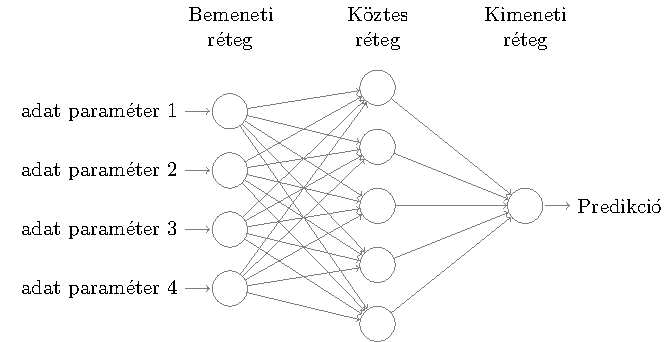
\includegraphics[height=40mm]{Figures/fig1.pdf}
\end{subfigure}\hspace{3.5 cm}
\begin{subfigure}[b]{0.3\textwidth}
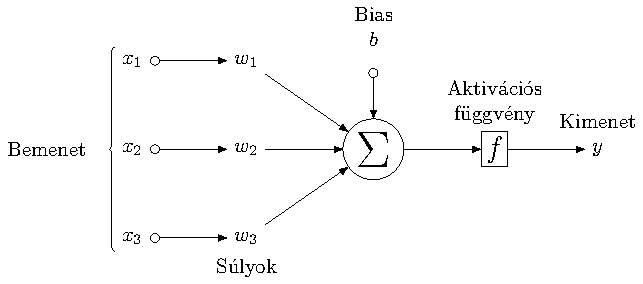
\includegraphics[height=35mm]{figures/fig2.pdf}
\end{subfigure}
\caption[Neurális háló vázlatos modellje]{Egy nerális háló vázlatos modellje és egy neuron aktivációjának a folyamata.}

\end{figure}
%%% fig1 end
Gyakran alkalmazott aktivációs függvény a sigmoid:
\begin{equation}
S(z) = \frac{1}{1 + e^{-z}}
\end{equation}
Illetve a \textit{rectified linear unit}(ReLU):
\begin{equation}
R(z) = \max{(0, z)}
\end{equation}
A ReLU előnye, hogy a súlyok optimalizálásánál történő deriválásoknál az eltünő gradiens problémája nem áll fenn, így gyorsabb tanulást eredményez és a sigmoidhoz képest nem olyan szűk intervallumon ad vissza értékeket. A bemenő adatok ilyen transzformációkon mennek keresztül, míg kimenő adatként össze lehet hasonlítani a várt kimenettel. Az összehasonlítás a hibafügvénnyel történik, ami kiszámolja a két érték közötti távolságot valamilyen metrikával. Legtöbbször a hibafüggvényt több különböző adat becslése után értékeltetjük ki, a háló \textit{batch}-okban kapja meg az adatot. Regressziós problémákban kedvelt hibafüggvény a \textit{mean sqared error}:
\begin{equation}
MSE = \frac{1}{n}\sum^n_{i =0}(y_i -p(x_i))^2
\end{equation}
a képletben a $p(x_i)$ az $x_i$ adatokból prediktált érték, $n$ pedig a \textit{batch} méret. A hiba minimalizálása egy optimalizációs probléma, a $p$ függvény a súlyoktól függ, amiket úgy kell megváltoztatni, hogy a hiba minimális legyen. A súlyok optimalizálása \textit{backpropagation}-nel történik, a hibafüggvényt deriválva a súlyok szerint a láncszabállyal, az utolsó rétegtől kezdve az elejéig, megkapjuk a gradiensmátrixokat rétegenként, amit szorozva egy kis számmal(\textit{learning rate}), levonva a súlymátrixokból megkapjuk az új súlyokat. A súlyok frissítése \textit{batch}-onként történik, így a \textit{batch}mérettel és a \textit{learning rate}-tel is lehet a tanulást gyorsítani, majd pontosabbá tenni \cite{batchs}.
%%% Architektúrák és CNN !!!
\newline\indent
A hálók architektúrájának kialakítására nincs általános szabály, intuíciónkra és hasonló problémámkon jól szereplő hálók mintájára kell hagyatkozni, tanulásából követkztetéseket levonni és alakítgatni. Általánosságban a komplexebb problémákhoz \textit{mélyebb}, több neuronból álló hálók kellenek, de ekkor a beállítandó paraméterek száma is nagyobb lesz, a tanítás lassabb lesz a megnövekedett számítási igény miatt. Képi adatoknál a paraméterek száma nagyon magas lenne, valamint a képnek nem az egész része érdekes, csupán részletek, és ezek a részletek bárhol lehetnek a képen, ezért nem célszerű teljesen összekötött neurális hálókat használni. Ezeknek a problémáknak a megoldására találták ki a konvolúciós neurális hálókat.
\newline\indent
A konvolúciós hálókban a rétegek között nincs teljes összeköttetés, a neuron csak az alatta lévő neuronnal, és annak szomszédaihoz kötődik. Az objektumfelismerő-osztályozó problémáknál az objektum bárhol előfordulhat a képen, ezért a neuronokat összekötő súlyoknak is eltolás invariánsank kell lennie, ezért egy rétegben minden neuron ugyanazokkal súlyokkal összegzi az allata lévő neuron szomszédainak kimenetét. A figyelembe vett szomszédok száma meghatároz egy \textit{filter} méretet, a \textit{filter} technikailag egy tenzor, aminek elemei a súlyok. A bemeneti képet végig páztázza a filter, és végrehajta az összegzéseket, az egyes kimenetek egy \textit{aktivációs térképet alkotnak}\footnote{szokásos feature map-nek is nevezni.}, amire alkalmazhatjuk a következő réteg konvolúciós réteget. Ez a műveleletet kétdimenziós diszkrét konvolúció a matematikában. A kimeneti \textit{aktivációs térkép} formája egy $n$ széles és hosszú, $c$ csatornával rendelkező képen alkalmazott $f\times f$ méretű, $s$ ugrással mintavételező \textit{filter}-rel, a képre $p$ \textit{padding}\footnote{kép szélén nullákkal létrehozott keret}-et alkalmazva a konvolúció során a következő képpen alakulnak:
\begin{equation}
a = \frac{n+2p-f}{s} +1,
\end{equation}
a képleteben $a$ létrejövő \textit{aktivációs térkép} szélessége, $k$ \textit{filter}t alkalmazva $a\times a\times k$ alakú \textit{aktivációs térképet} kapunk. Az \textit{aktivációs téképek} méretét csökkenteni kell az első kettő dimenziójában, $k$ a \textit{filterek} számával lesz egyenlő. Erre egy módszer a \textit{pooling}. A $poolingoknak$ sok fajtája van, legnépszerűbb a \textit{Maxpooling} és az \textit{AveragePooling}, alapja, hogy a \textit{filterek}hez hasonlóan végig pásztázza a képet egy \textit{kernel},  \textit{Maxpooling} esetében a kernel méreten belüli elemek közül a maximális nagyságút adja át az \textit{aktivációs térképnek}, \textit{Averagepoolingnál} pedig a kernelen belüli elemek átlagát adja át.
\section{Eddigi eredmények és módszerek áttekintése}
%%% irodalmi áttekintés az image---> redshift és eredményeik.


 \chapter{Adatok}
 Az eredményes gépi tanuláshoz a nagy mennyiségű és jó minőségű adat majdnem annyira fontos, mint a jó modell megválasztása. Általában nem áll  rendelkezésünkre egyből az algoritmusnak adható adat, a nyers adatokat előbb preprocesszállni kell, ki kell nyerni a fontos tulajdonságokat, melyek előztetes ismereteink alapján fontosak lehetnek, és össze kell állítani az adathalmazt, amelyet majd  szétválasztunk tanuló- és teszthalmazra. 
 \newline \indent 
 A kutatómunkámhoz sok, jó minőségű galaxis képére volt szükségem, és mindegyik galaxisnak a spektroszkópiával mért vöröseltolódására is, ezekhez az adatokhoz a Sloan Digital Sky Survey adatbázisában fértem hozzá.
 
\section{Sloan Digital Sky Survey}
 A Sloan Digital Sky Survey az eddigi legrészletesebb égboltfelmérés, mély, több színsávos képekkel az ég egyharmadáról, 500 milló asztrofizikai objektumról, 3 millió felvett spektrumadattal. A felmérést 2000-ben kezdte, több ciklusban, 2014-ben kezdődőtt a negyedik fázis (SDSS-IV), és már elkezdődtek a megbeszélések az SDSS-V elindításáról\cite{sdssV}. A megfigyelési adatokat egy külön erre a célra megépített 2.5 m széles optikai teleszkóp szolgáltatja az Apache Point Obszervatóriumból, Új Mexikóban.
 Öt színsávaban mér, a látható fény és az infravörös tartománya között,  $u$, $g$, $r$, $i$ és $z$ színszűrőkkel (ultraviolet, green, red, near infrared és infrared), amik 3000 \AA\text{ }  és 10000 \AA\text{ }  közötti tartományt fedik le. A különböző szűrőkön keresztül a CCD chipek egymás után rögzítenek, 71.2 másodperc késéssel, $r$, $i$, $u$, $z$ és $g$ sorrendben, így a különböző színű képeken előfordulhat, hogy egy objektum kicsivel arrébb. Ennek volt előnye is, mozgó objektumokat könnyebben lehetett azonosítani, például létre tudtak hozni aszteroida katalógusokat. Az SDSS képek alapvető egysége a \textit{field}, ami 10-szer 13 szögperces szeletet tartalmaz az égből, és 1489-szer 2048 pixelt tartalmaz és az egyes \textit{fieldeket} három jelzőszám teszi egyedivé, a \textit{field number},  a \textit{run}, ami a szkennelés száma, a \textit{camera cloumn}, ami a megmutatja melyik oszlop CCD kamera készítette a képet egy 1 és 6 közötti szám, mindegyik oszlop egy \textit{fieldet} készít, ami 128 pixel szélességben fed át a szomszédossal.  Az elkészült felvételek az SDSS képfeldolgozó pipelinejába kerülnek, ahol kalibrált FITS formátumú képet csinálnak, és a katalógushoz hozzá adják a képi paramétereket.
 \newline \indent
 A megfigyeléseket folyamatosan végzik, az adatbázisokat viszont csak évente frissítik, ezeket a \textit{data release}-nek (DR) hívják és tartalmazzák az előző megfigyelésekből származó adatokat is. Az SDSS virtuális oszervatórium keretrendszerben működik, adatai publikusak. Az objekumok és paramétereik relációs adatbázisba vannak rendezve, a SQL nyelvet használva lehet lekérdezéseket indítani.
 %%%% Casjobs és sciserver
 \section{A tanítóhalmaz elkészítése}
 A tanítóhalmaz elkészítését a \textit{SciServeren}\cite{sci} végeztem, amely \textit{Jupyter Notebook} keretrendszerben nyújtott adatfeldolgozó és számoló felületet, valamint közvetlen elérést az SDSS \textit{DR7}-es \textit{fieldekhez}. A szerveren egy \textit{API} segítségével közvetlenül lehetett \textit{python} környezetben SQL lekérdezéseket végezni az SDSS adatbázisából, az így kapott táblákat elmenteni. Két tanítóhalmazt állítottam össze, az 1-es adathalmaz $\num{150000}$ képből áll, a galaxisok mindegyik színszűrőn mért magnitúdója $15^m$-nál halványabb és $22^m$-nál fényesebb. A legtöbbször ezt az adathalmazt használtam tanításra és tesztelésre, viszont a vöröseltolódás-eloszlásában lévő csúcs miatt létrehoztam egy 2-es adathalmazt is, melyben a vöröseltolódás eloszlás
 kicsit egyenletesebb létrehozása során nem csináltam felső határt a magnitúdónak, de a vöröseltolódásokat határok közé szorítottam, több lekérdezés eredményéből állt össze az adattábla,.
  \newline \indent
Feltételként szabtam meg, hogy a galaxisok vöröseltolódás $0.05$-nél nagyobb legyen, hogy a nagy fényességük miatt a képeken szaturációt okozó csillagok ne keveredjenek bele, valamint $1$-nél kisebb legyen a vöröseltolódás, hogy az SDSS adatbázisában tévesen galaxisnak osztályozott kvazárok se kerüljenek bele. A képméret kiválasztásánál figyelembe kellett venni, hogy a túl nagy kép túl sok haszontalan információt is tartalmazhat, valamint a közeli szomszédos objektumok is félrevezethetik a neurális hálót, de a túlságosan kicsi képméret miatt lehet lemarad fontos információ. Ezért vizualizálva a galaxisokat különböző képmérettel, az optimális választásnak az $50\times 50$ pixeles méret tűnt.
\newline\indent
 A \textit{SciServer}-en az egyes \textit{field}ek olyan könyvtárstruktúrába vannak rendezve, hogy a \textit{run, rerun, camcol, fieldID} és színszűrő alapján kereshetőek. 
 Ezért az SQL lekérdezésnél a magnitúdó, vöröseltolódás és objektum azonosító addatai mellett lekérdeztem \textit{field} könyvtárban megtalálásához szükséges adatokat, valamint az egyes színszűrőkkel készített képen hol van a galaxis közepe\footnote{sor és oszlop pixelben, a különböző színszűrőkön készített képeken  máshol volt az objektum közepe a SDSS képalkotása miatt.}. A galaxis közepének lehelyezkedésére az volt a kikötés, hogy ne a kép szélének $25$ pixeles szomszédságában helyezkedjen el, így a kivágásnál nem fog gondot okozni a hiányzó információ. Az így kapott táblákkal előtudtam hívni a FITS formátumú \textit{field}eket, melyekből ki tudtam vágni a galaxis $50\times 50$ méretű képét, levontam a \textit{Softbias}-t\footnote{a \textit{fieldek}hez hozzáadtak egy 1000-es nagyságrendű számot a kép készülése után, hogy ne legyen negatív pixelérték sehol.}, és az eredeti könyvtárstruktúrához hasonló módon elmentettem a képet, egy \textit{python dictionarybe} pedig az elérési útvonalat és az objektum azonosítóját, így azonosító alapján előhívható volt a kivágott kép. Ezt mindegyik szűrővel készült képre külön megcsináltam, majd az összes képet egy nagy tömbbe tettem a könnyebb mozgatás és elérés érdekében. A tömb dimenziója $\text{objektumok száma}\times \num{12500}$ lett, a különböző színű, azonos objektumról készült képeket egymás után tettem, így az adatokat tartalmazó tábla sorának sorszámával lehetett megtalálni a képeket. Ez a tárolási mód okozhatna olyan hibát, hogy elcsúsznak, és nem a megfelelő indexnál lesznek a képek, de ezt véletlen mintavételezéssel megjelenítve a képet és az azonosítót, össze tudtam hasonlítani az SDSS képeivel. A képi adattömb az 1-es adathalmazhoz 14GB méretű lett,  aminek a betöltéséhez nagy memóriájú gép kellett, a betöltött tömb formája már könnyen alakítható volt a feladat igényeihez. %Megjegyezendő, hogy a tanítóhalmaz elkészítése gyorsítható, ha a megnyitott \textit{field}eket nem zárjuk be miután egy objektumot kivágtunk, hanem a táblában még szereplő azonos \textit{field}ű galaxisokat is kivágjuk, és csa utána csukjuk be.
 
 
 \section{Adatexploráció}
 Mielőtt elkezdenénk a tanítást, érdemes megvizsgálni a tanulóhalmazunk statisztikai jellemzőit, megnézni mennyire jól reprezentálja a valóságot, valamint feltárni az  összefüggéseket. Ehhez az SDSS \textit{DR7}-es adatbázisának vöröseltolódás-eloszlásával hasonlítottam össze a tanulóhalmaz eloszlását, alkalmaztam egy \textit{Random Forest regreesort} az \textit{ugriz} magnitúdóértékekre, és készítettem egy \textit{korrelációs térképet} a magnitúdókkal és vöröseltolódásokkal. 
 \newline\indent
 Az SDSS \textit{DR7}-ben a galaxisok vöröseltolódásának mediánja $z\sim0.07$ \cite{rsd}, a teszthalmazomé $z\sim0.11$, ami a 0.05-ös vöröseltolódásbeli vágásomnak tudható be.  
 \begin{figure}[h!]
 \centering
  \begin{subfigure}[b]{0.35\textwidth}
    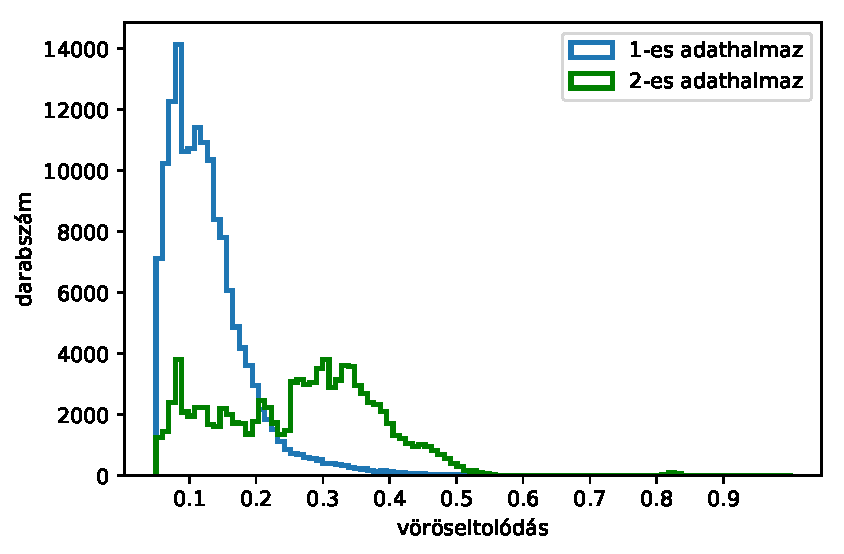
\includegraphics[width=\textwidth, height = \textwidth]{Figures/hists.pdf}
    %\caption{Picture 1}
    \label{fig:1}
  \end{subfigure}
  \hspace{2cm}
  \begin{subfigure}[b]{0.35\textwidth}
    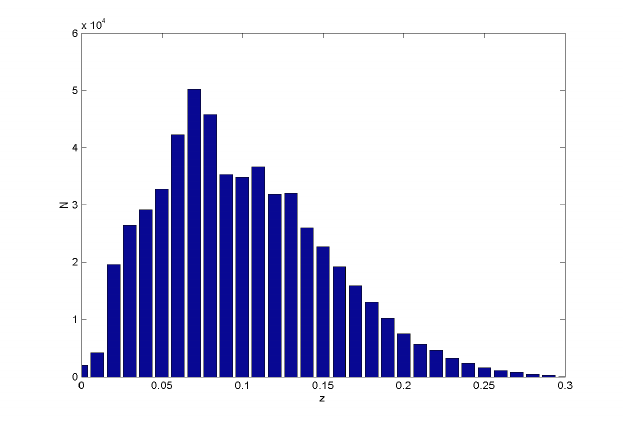
\includegraphics[width=\textwidth, height = 1.05\textwidth]{Figures/rsd.png}
    \label{fig:2}
  \end{subfigure}
  \caption{Az általam előállított tanulóhalmaz és az SDSS \textit{DR7} vöröseltolódás-eloszlása. A jobboldali kép forrása: \cite{rsd}}
  \label{fig:dist}
 \end{figure}
 Összehasonlítva a \ref{fig:dist}. ábrán a baloldalon az 1-es adathalmaz hisztogramját a jobboldalival, a két eloszlás jó hasonlóságot mutat, a vágásban van különbség, a legtöbb galaxisnak mind a kettő esetben 0.3-nál kisebb a vöröseltolódása. .

 \begin{figure}[]
 \centering
  \begin{subfigure}[b]{0.32\textwidth}
    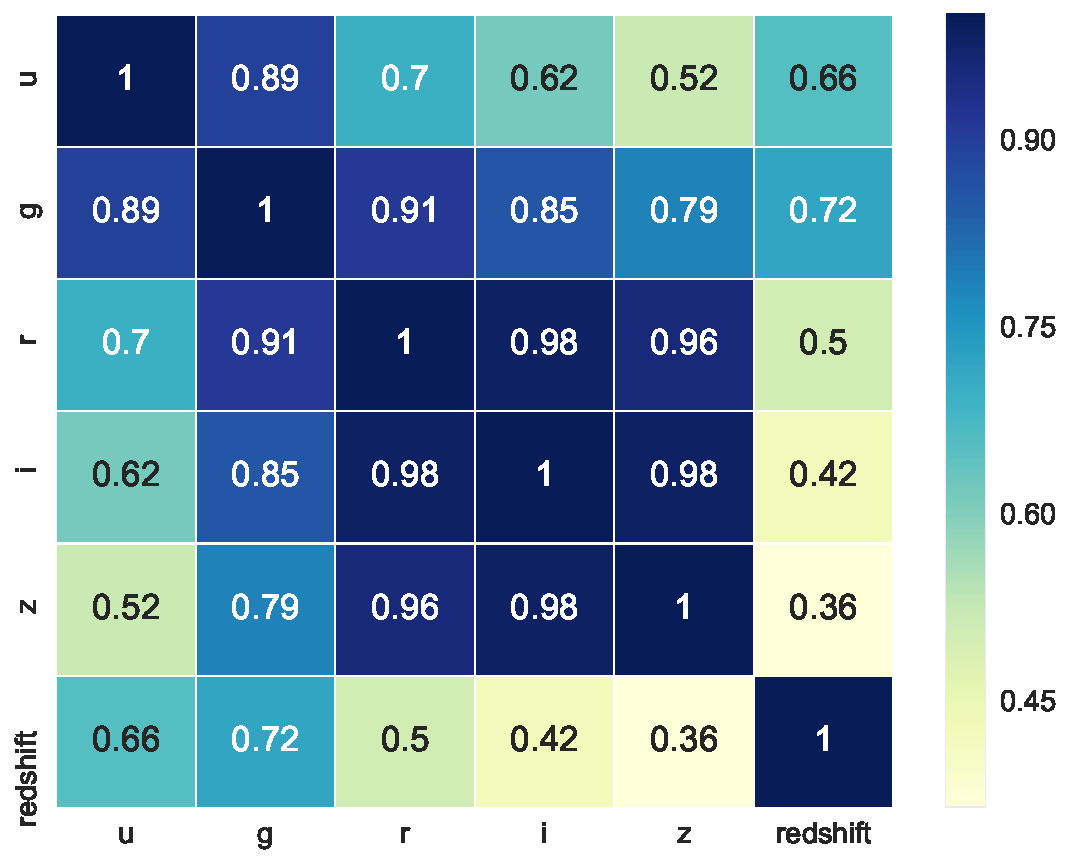
\includegraphics[width=\textwidth, height = \textwidth]{Figures/corrmap.pdf}
    %\caption{Picture 1}
    \label{fig:1}
  \end{subfigure}
  \hspace{0cm}
  \begin{subfigure}[b]{0.32\textwidth}
    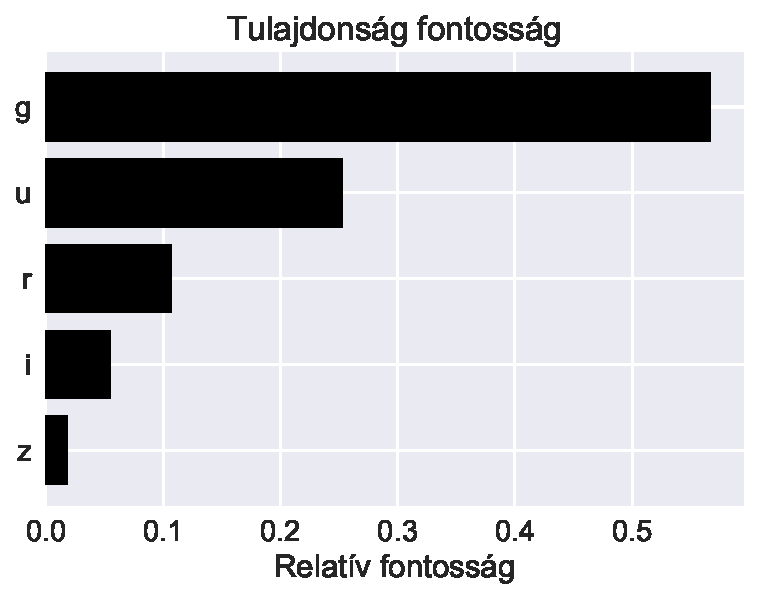
\includegraphics[width=\textwidth, height = \textwidth]{Figures/relf.pdf}
    \label{fig:2}
  \end{subfigure}
  \hspace{0cm}
  \begin{subfigure}[b]{0.32\textwidth}
    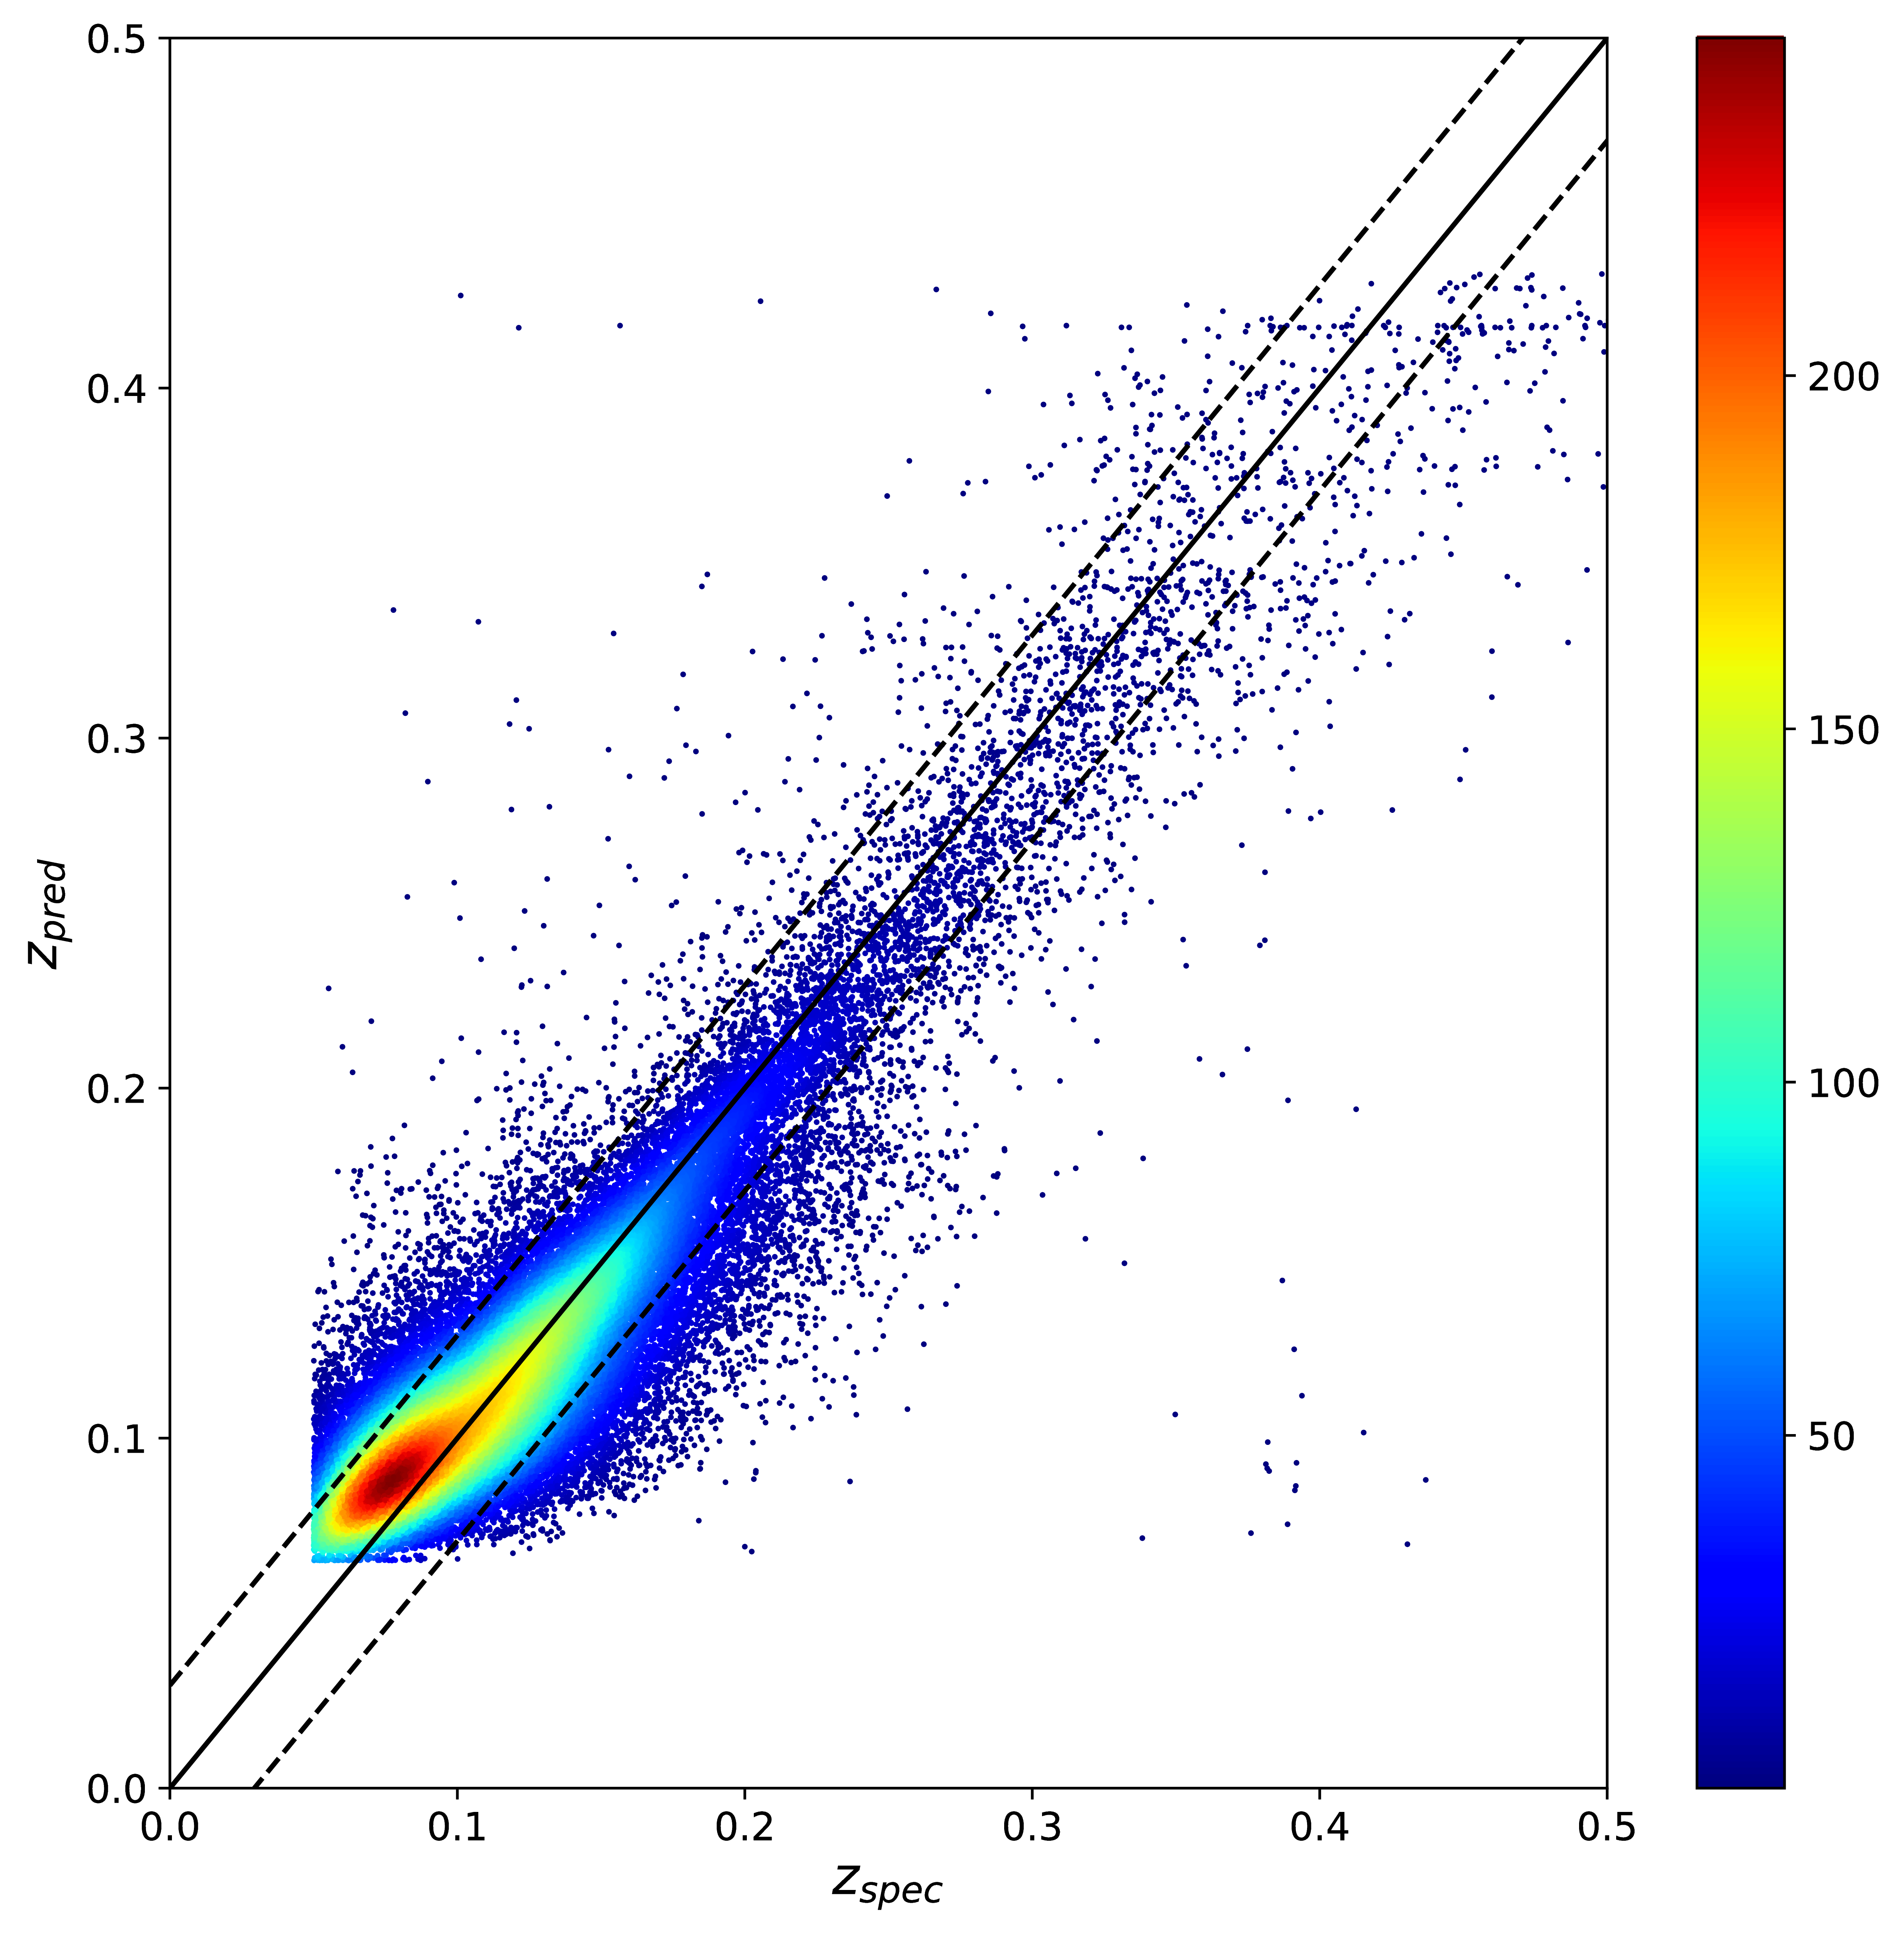
\includegraphics[width=\textwidth, height = 0.95\textwidth]{Figures/plotbaselineRF.png}
    \label{fig:2}
  \end{subfigure}
  \caption{A \textit{korrelációs mátrix},a \textit{Random forest} tanulásában a különböző tulajdonságok relatív fontossága és a magnitúdókból becslése. A szaggatott vonal a \textit{rmse} nagyságát ábrázolja.}
  \label{fig:dist2}
 \end{figure}
A korrelációs mátrix elemeiből az látszik, hogy az egymás melletti színek magnitúdója erősen korrelál a szomszédossal. A magnitúdok és a vöröseltolódás nem korrelál ilyen szinten, legmagasabb korrelációs együtthatója a \textit{g} magnitúdoknak van a vöröseltolódással. Ezek után alaklmaztam az adatok közül az első $\num{100000}$-re a \textit{Random forest}-et, majd prediktáltattam az utolsó $\num{50000}$ mintán. A véletlen erdő $rmse =0.029$ jósággal prediktált, a becsült vöröseltolódás-értékekeket a \ref{fig:dist2} ábra bal szélén ábrázoltam a spektroszkópiai vöröseltolódások függvényében. Az ábrán látható, hogy a pontok nagyrésze ráfekszik az ideálist jelző vonalra, viszont ahol a legsűrűbb a pontok elhelyezkedése, szisztematikus hibája van a rendszernek, felül becsül. A legfontosabb paraméternek a becslés során a \textit{g} magnitúdóérték bizonyult, ennek relatív fontossága $0.59$ volt, ami jóval magasabb, mint a második legfontosabb \textit{u} értéknek, ami $0.24$. A tulajdonságok relatív fontosságának sorrendje összhangban van az egyes fényeségek vöröseltolódással vett korrelációjával.
 \newline\indent
 A magnitúdó adatok elemzése azért indokolt, mert a bemeneti adataink az öt csatornás képek lesznek, és a magnitúdók az egyes csatornákhoz köthető származtatott adatok. A legtöbb gépi tanuláson alapuló vöröseltolódás-becslő módszer ezeket az adatokat használja, ezért ha a képekből ki tudjuk nyerni gépi tanulással megfelelő pontossággal a fényességértékeket, alkalmazhatunk már bevált módszert rá.
 
 
 \chapter{Módszerek és eredmények}
 A kutatáshoz az egyes gépi tanulási módszereket \textit{python} nyelven a \textit{keras} (neurális hálók) és \textit{sci-kit learn} (\textit{random forest}) könyvtárakkal valósítottam meg. A tanulás gyorsítása érdekében a tanítást a \textit{Google Cloud} felhő alapú számítási szolgáltatást nyújtó platformon végeztem NVIDIA Tesla K80-as GPU-val.
 
 

\section{Neurális hálók és Random Forest kombinálva}
A \textit{random forest} algoritmus jól teljesít a magnitúdókból prediktálás során, így célszerű megvizsgálni, hogy mennyire működik jól, ha a magnitúdóértékek is becslésből származnak. A képekből való fényességbecsléshez mind az öt színszűrőhöz elkészítettem egy-egy konvoluciós neurális hálót, ezeket a hálókat az első $\num{50000}$ képen tanítottam be. A következő $\num{50000}$ képpel prediktáltam magnitúdóértékeket, ezeket a becsült magnitúdókat használtam, a \textit{random forest regressor} tanításához. A harmadik $\num{50000}$ képnek is megbecsültem a magnitúdóit, és ezekből predikált a véletlen erdő vöröseltolódás-értékeket, így nem volt átfedés a tanuló-és teszthalmazok között. A neurális hálók tanításánál 80 \textit{epoch}-ot használtam mindegyik hálóra, de nem egyben ment végig a tanulás, a \textit{learning rate}-t csökkentettem, ha a hibafüggvény értéke nem csökkent, illetve a \textit{batch} méretet is növeltem közben. Az egymás melletti\footnote{hulámhossz szerint} magnitúdók korrellálása, illetve a célváltozók és a bemeneti adatok hasonlóság miatt az volt a feltételezésem, hogy ugyanolyan architektúrájú neurális hálókat lehet használni mindegyik fényességérték számításához.
\newline\indent
Az egyes hálók bemenetként megkapták az $50\times 50\times 1$ méretű, az adott színszűrőn keresztül készített képet inputként. Az első réteg egy konvolúciós réteg volt, $32$ darab $2\times 2$-es filterből állt, alkalmaztam rá a \textit{ReLu} aktivációt és utána egyből egy $2\times 2$ \textit{MaxPooling}-ot.
%%%%%%%%% FIGURES %%%%%%%%%%
\begin{figure}[]
  \begin{subfigure}[b]{0.3\textwidth}
    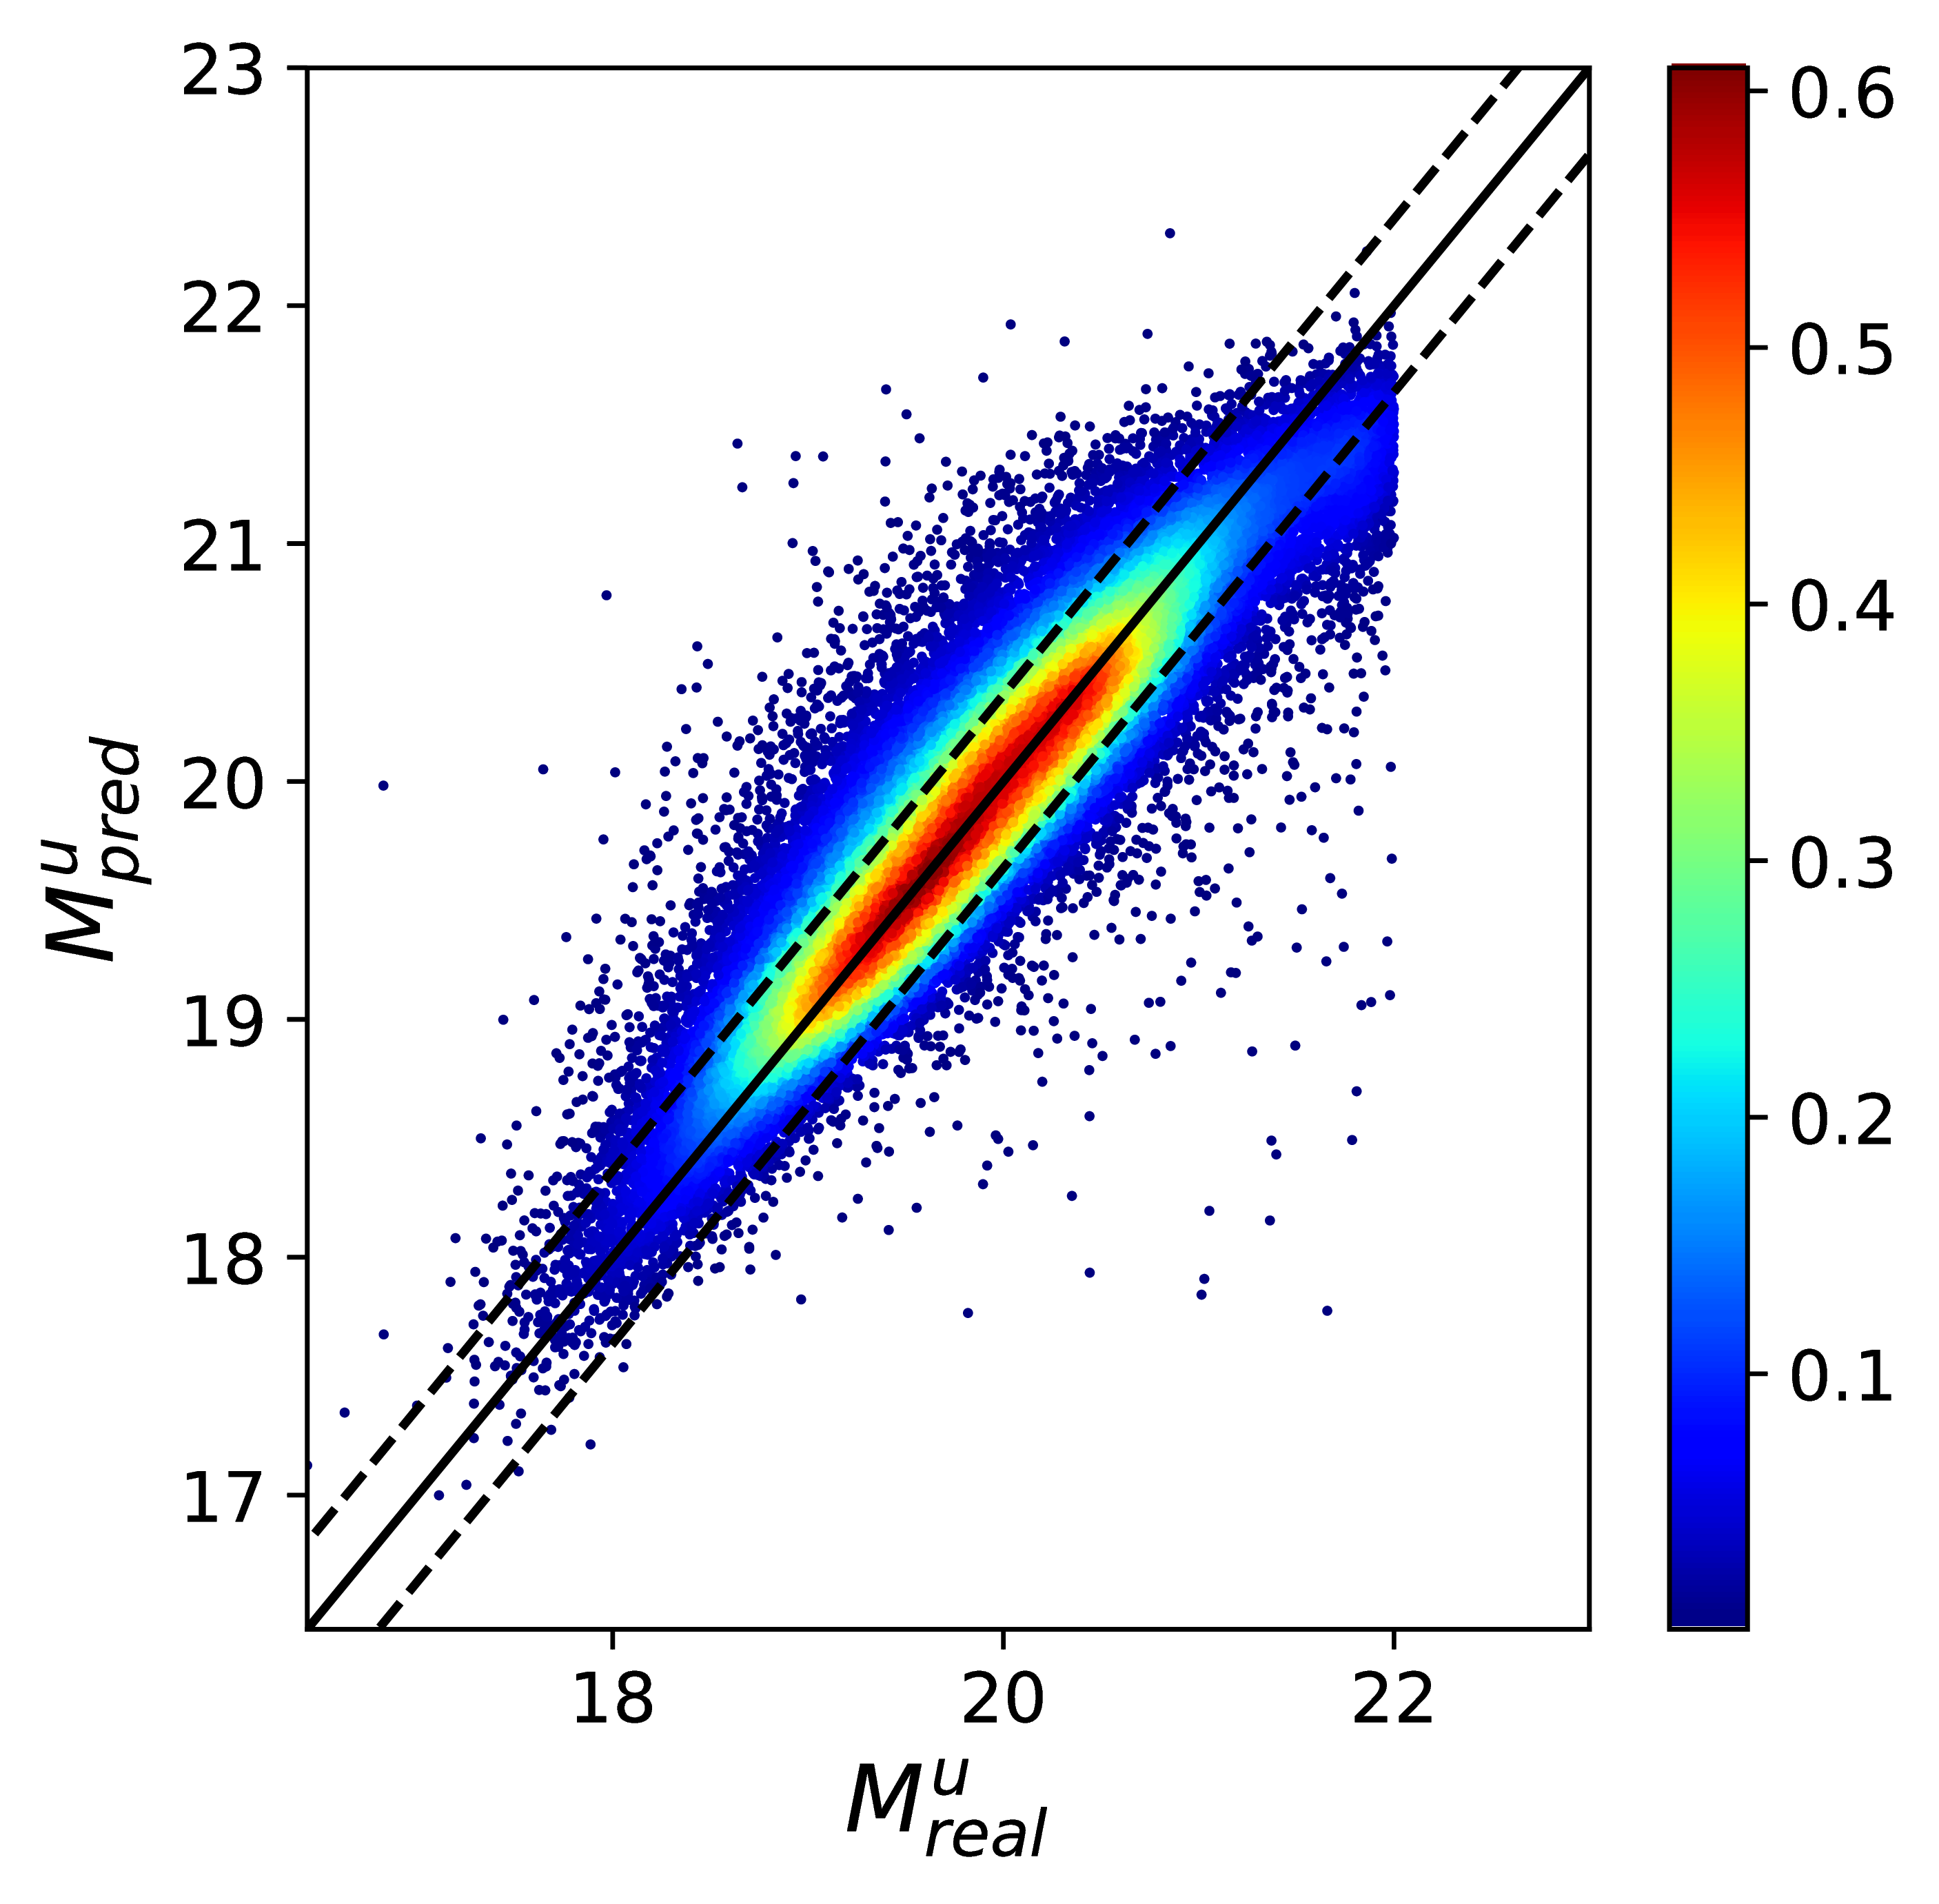
\includegraphics[width=\textwidth, height = \textwidth]{Figures/pmu3.png}
    %\caption{Picture 1}
    \label{fig:1}
  \end{subfigure}
  \hspace{0cm}
  \begin{subfigure}[b]{0.3\textwidth}
    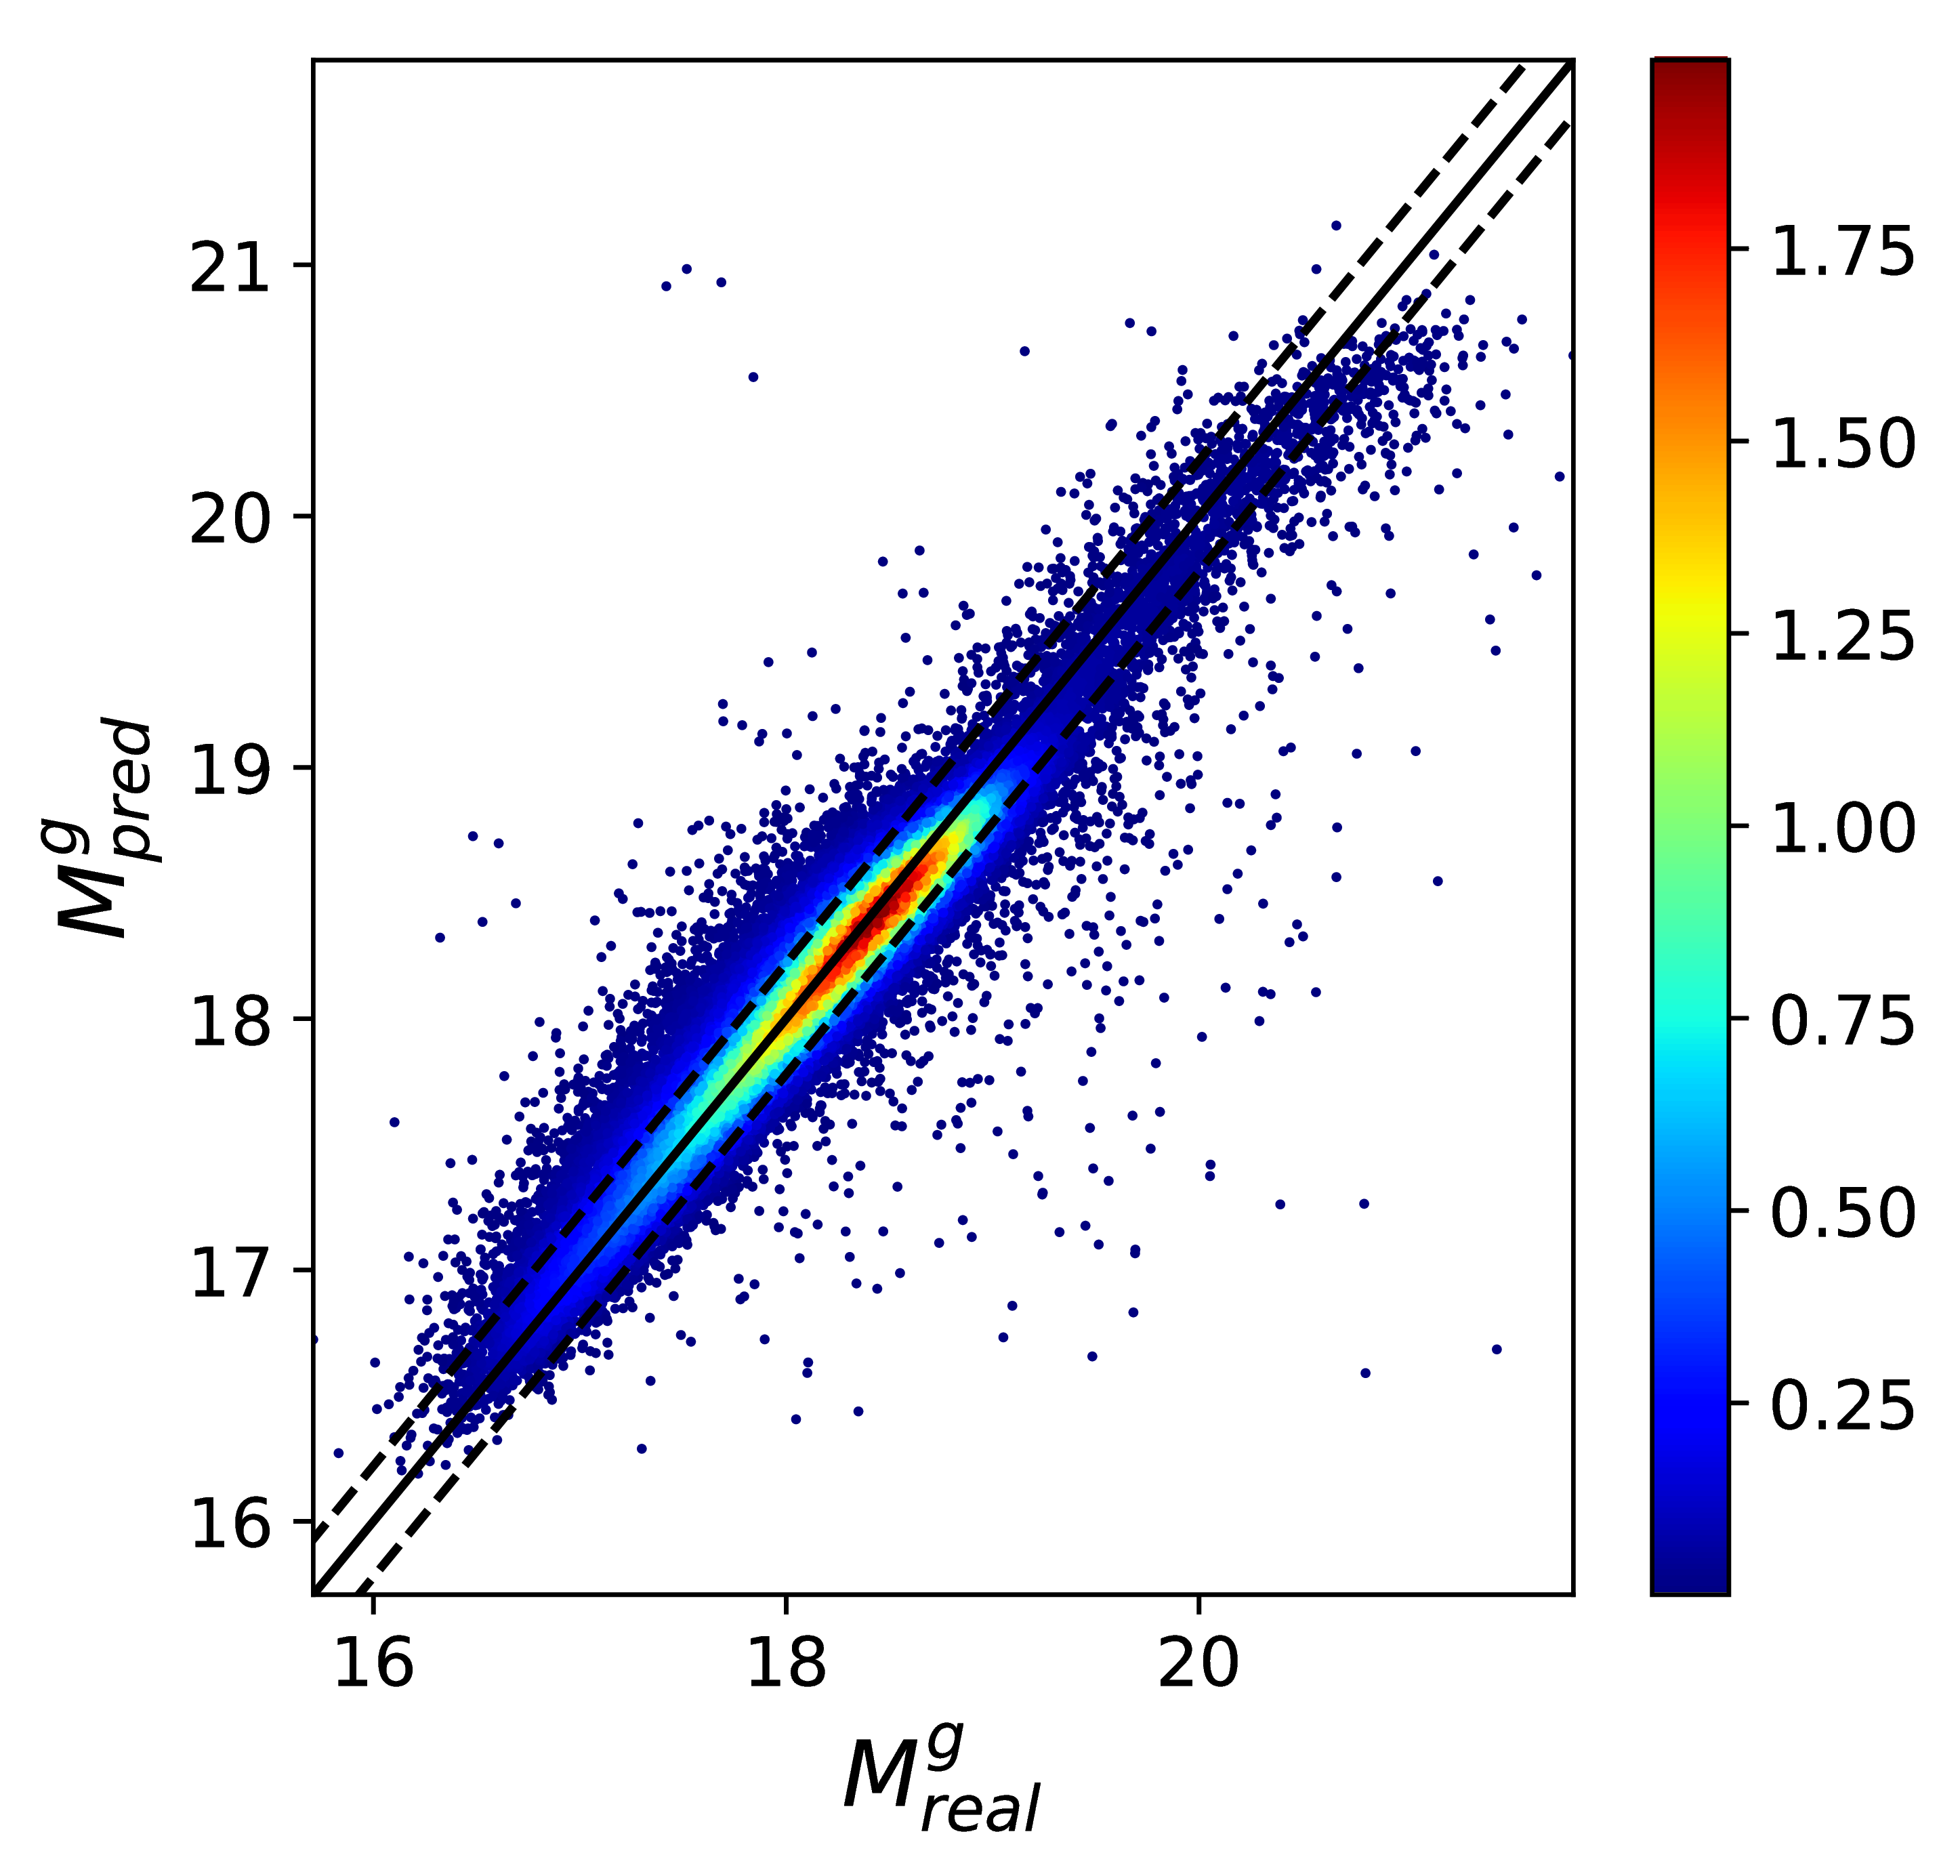
\includegraphics[width=\textwidth, height = \textwidth]{Figures/pmg3.png}
    \label{fig:2}
  \end{subfigure}
  \hspace{0cm}
  \begin{subfigure}[b]{0.3\textwidth}
    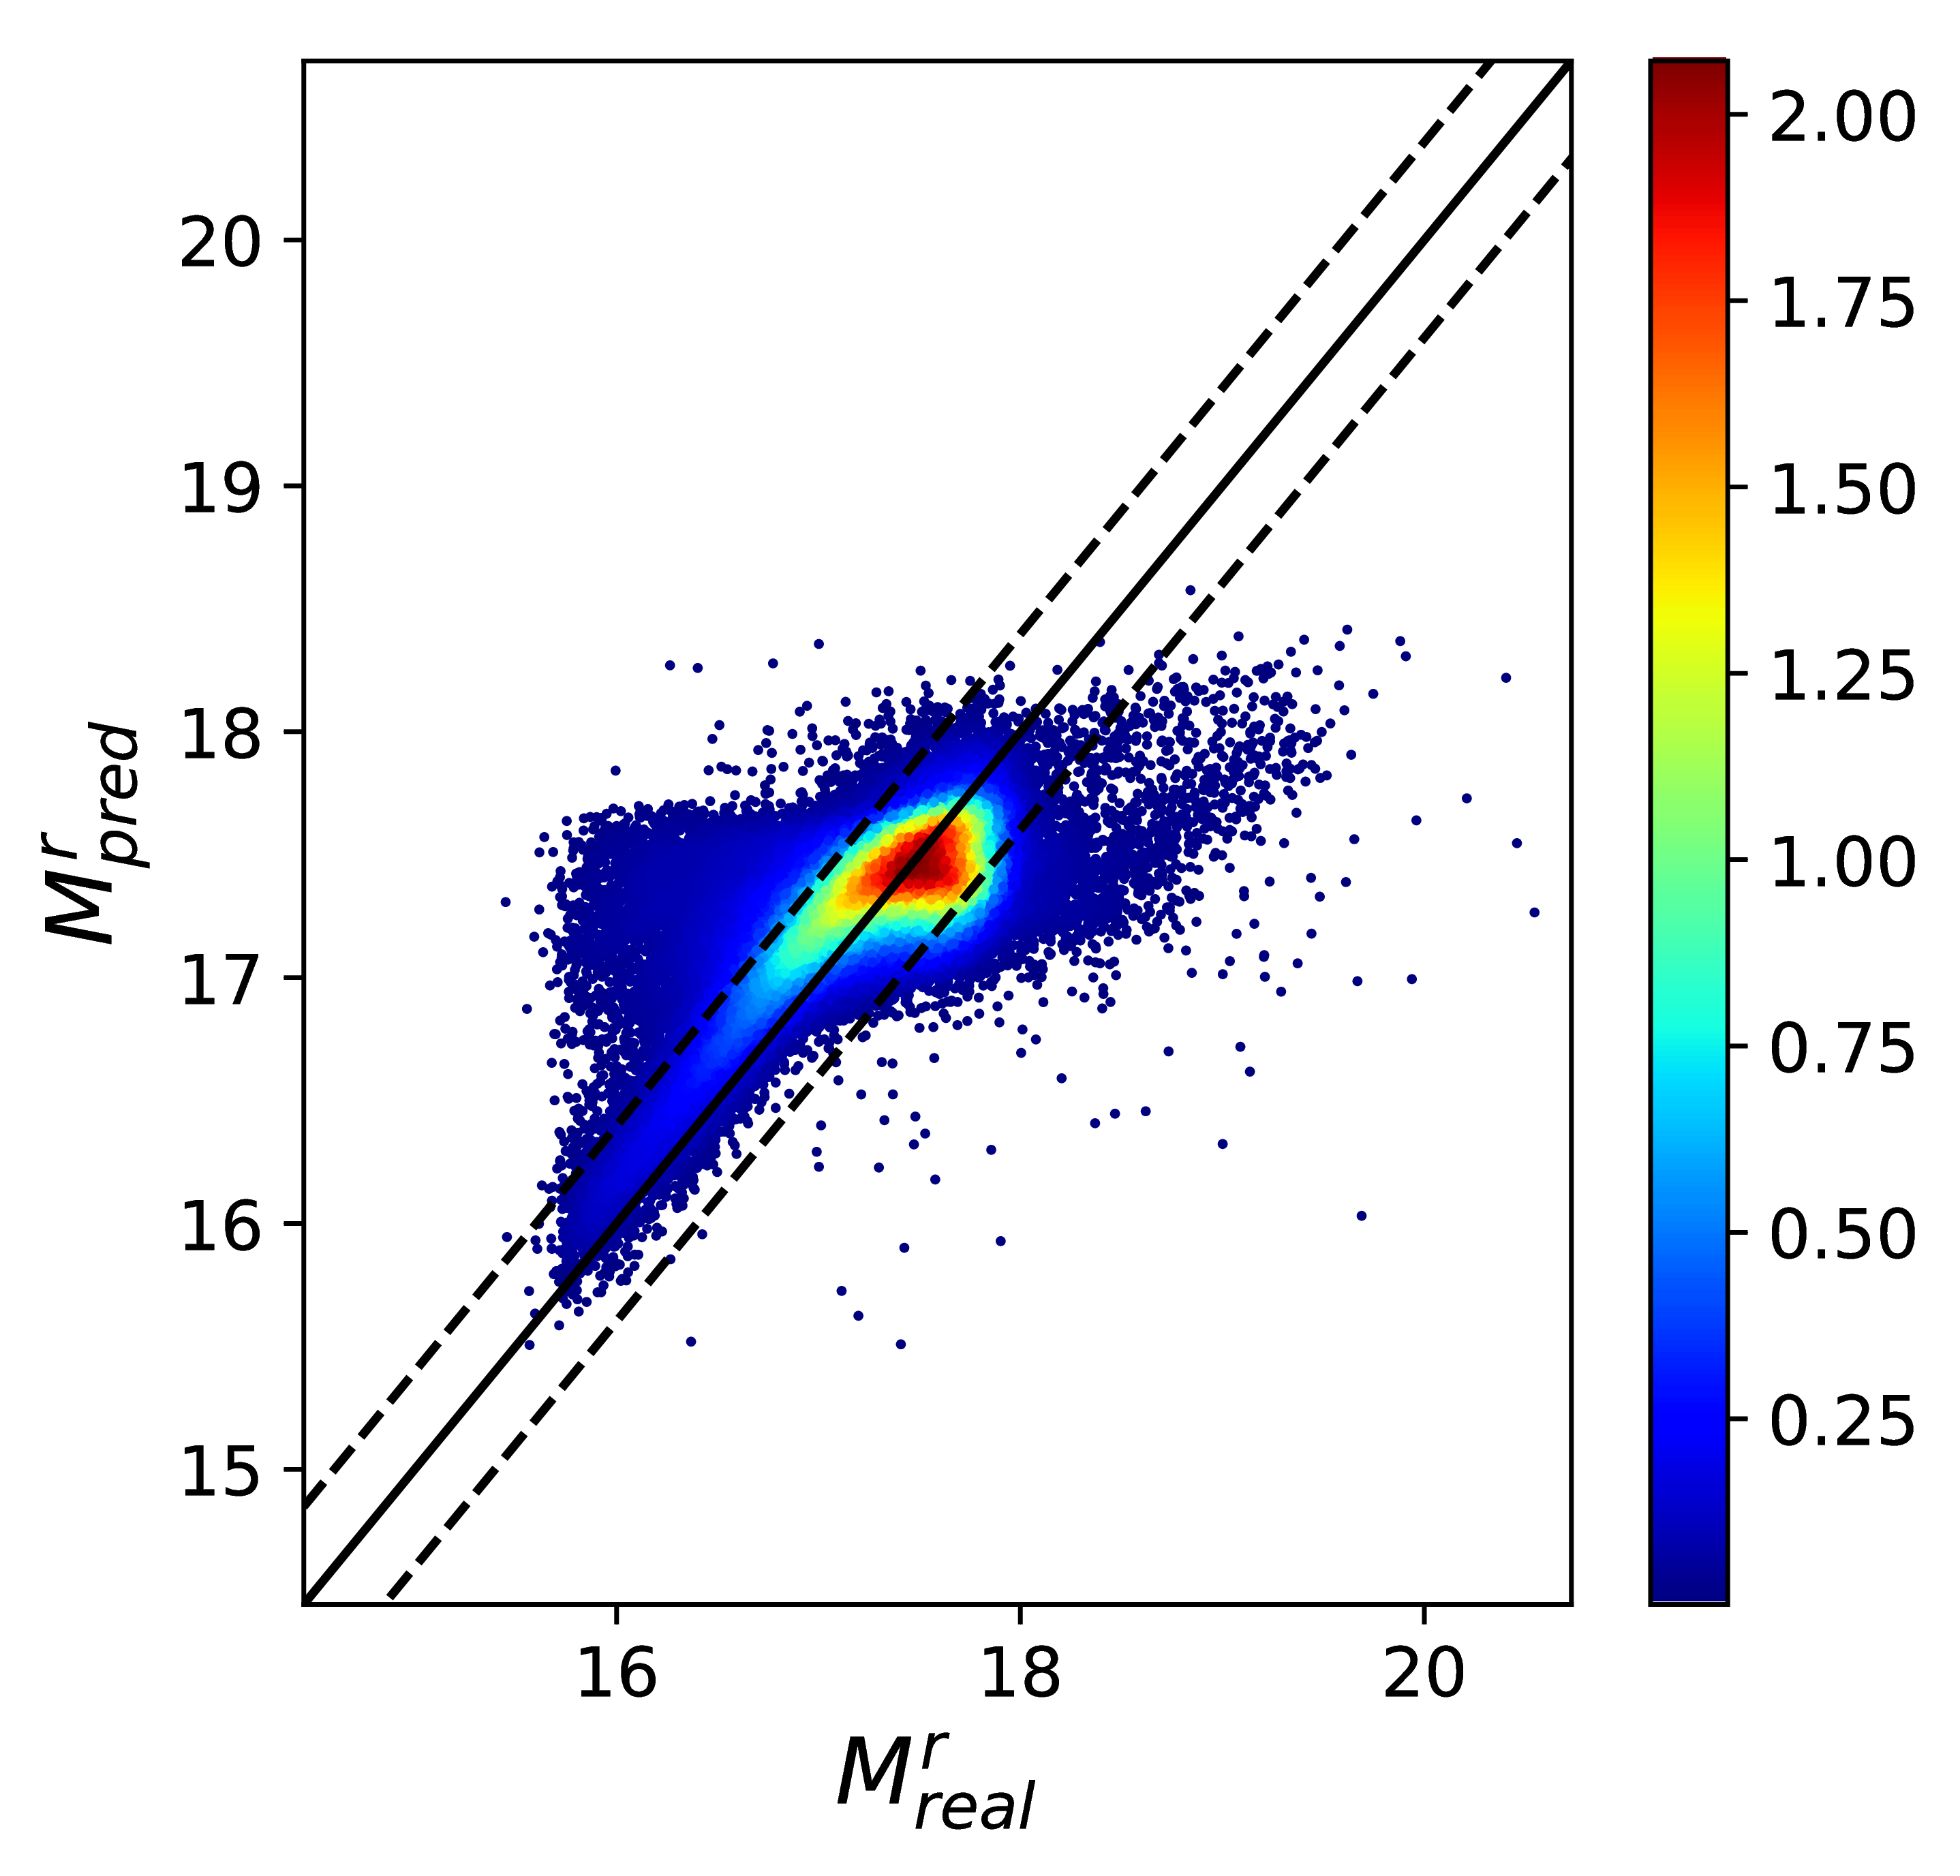
\includegraphics[width=\textwidth, height = \textwidth]{Figures/pmr3.png}
    \label{fig:2}
    \hspace{0cm}
  \end{subfigure}
  \centering
   \begin{subfigure}[b]{0.3\textwidth}
    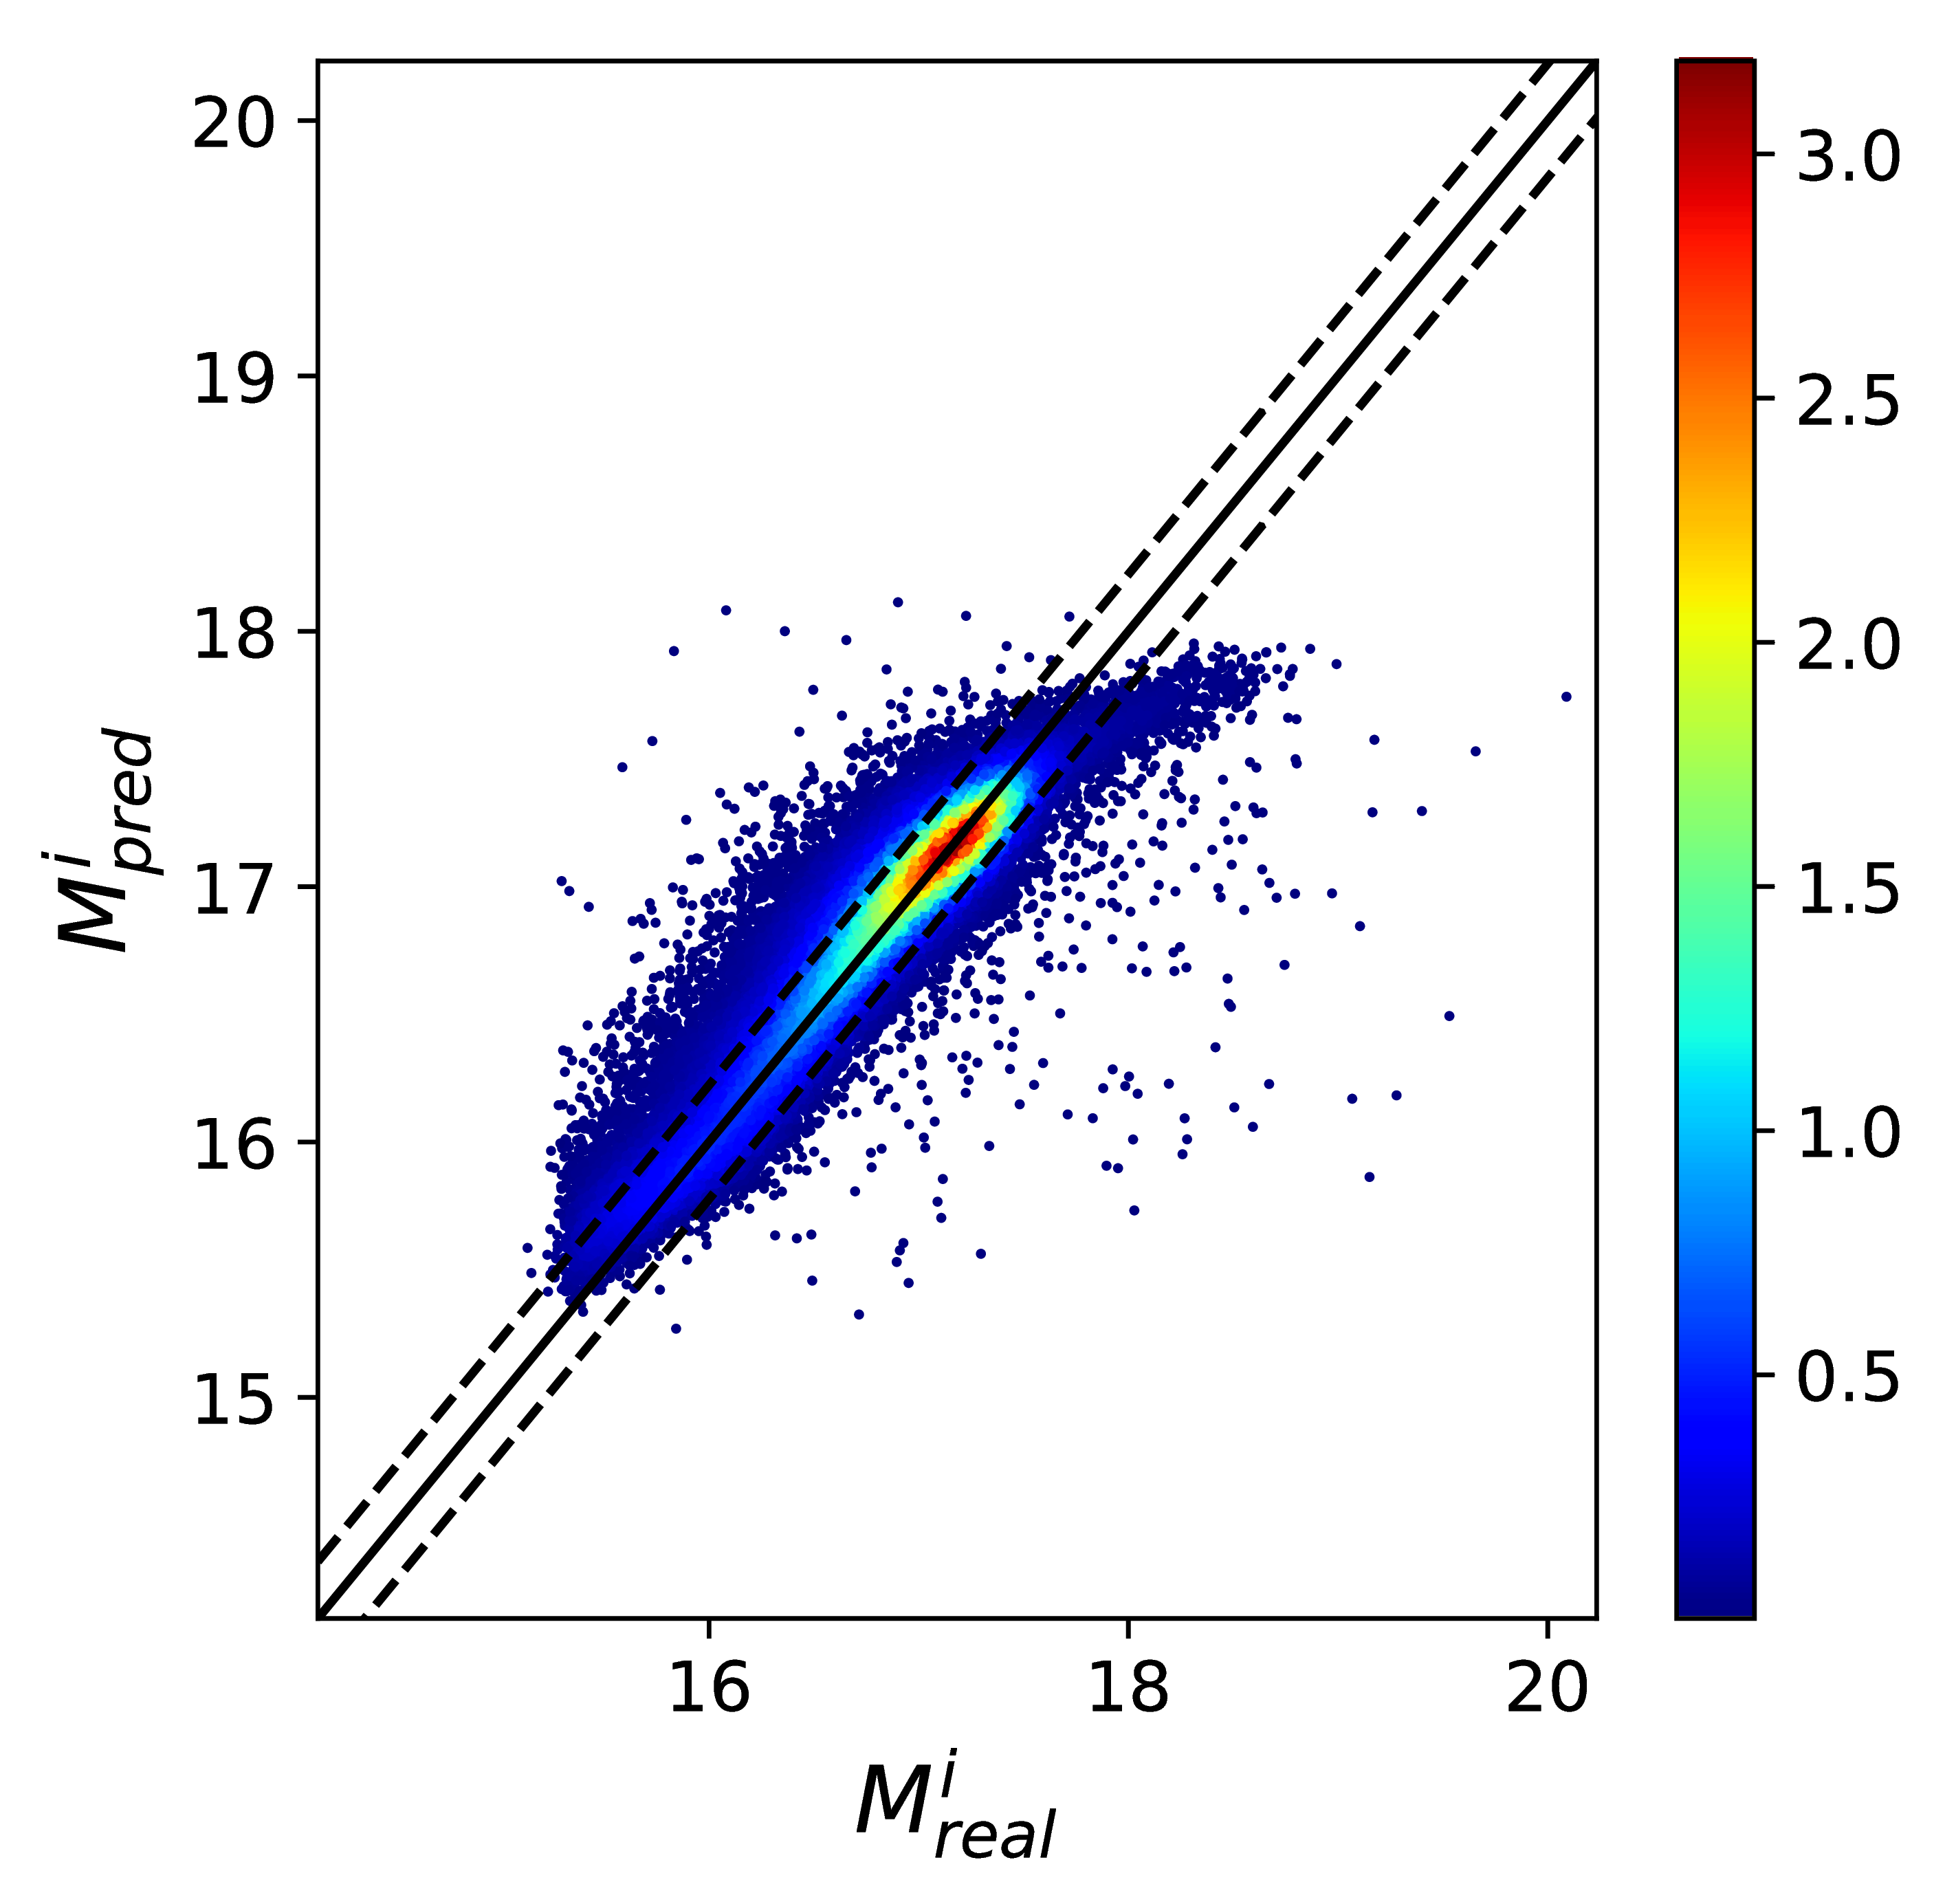
\includegraphics[width=\textwidth, height = \textwidth]{Figures/pmi3.png}
    \label{fig:2}
    \hspace{0cm}
  \end{subfigure}
   \begin{subfigure}[b]{0.3\textwidth}
    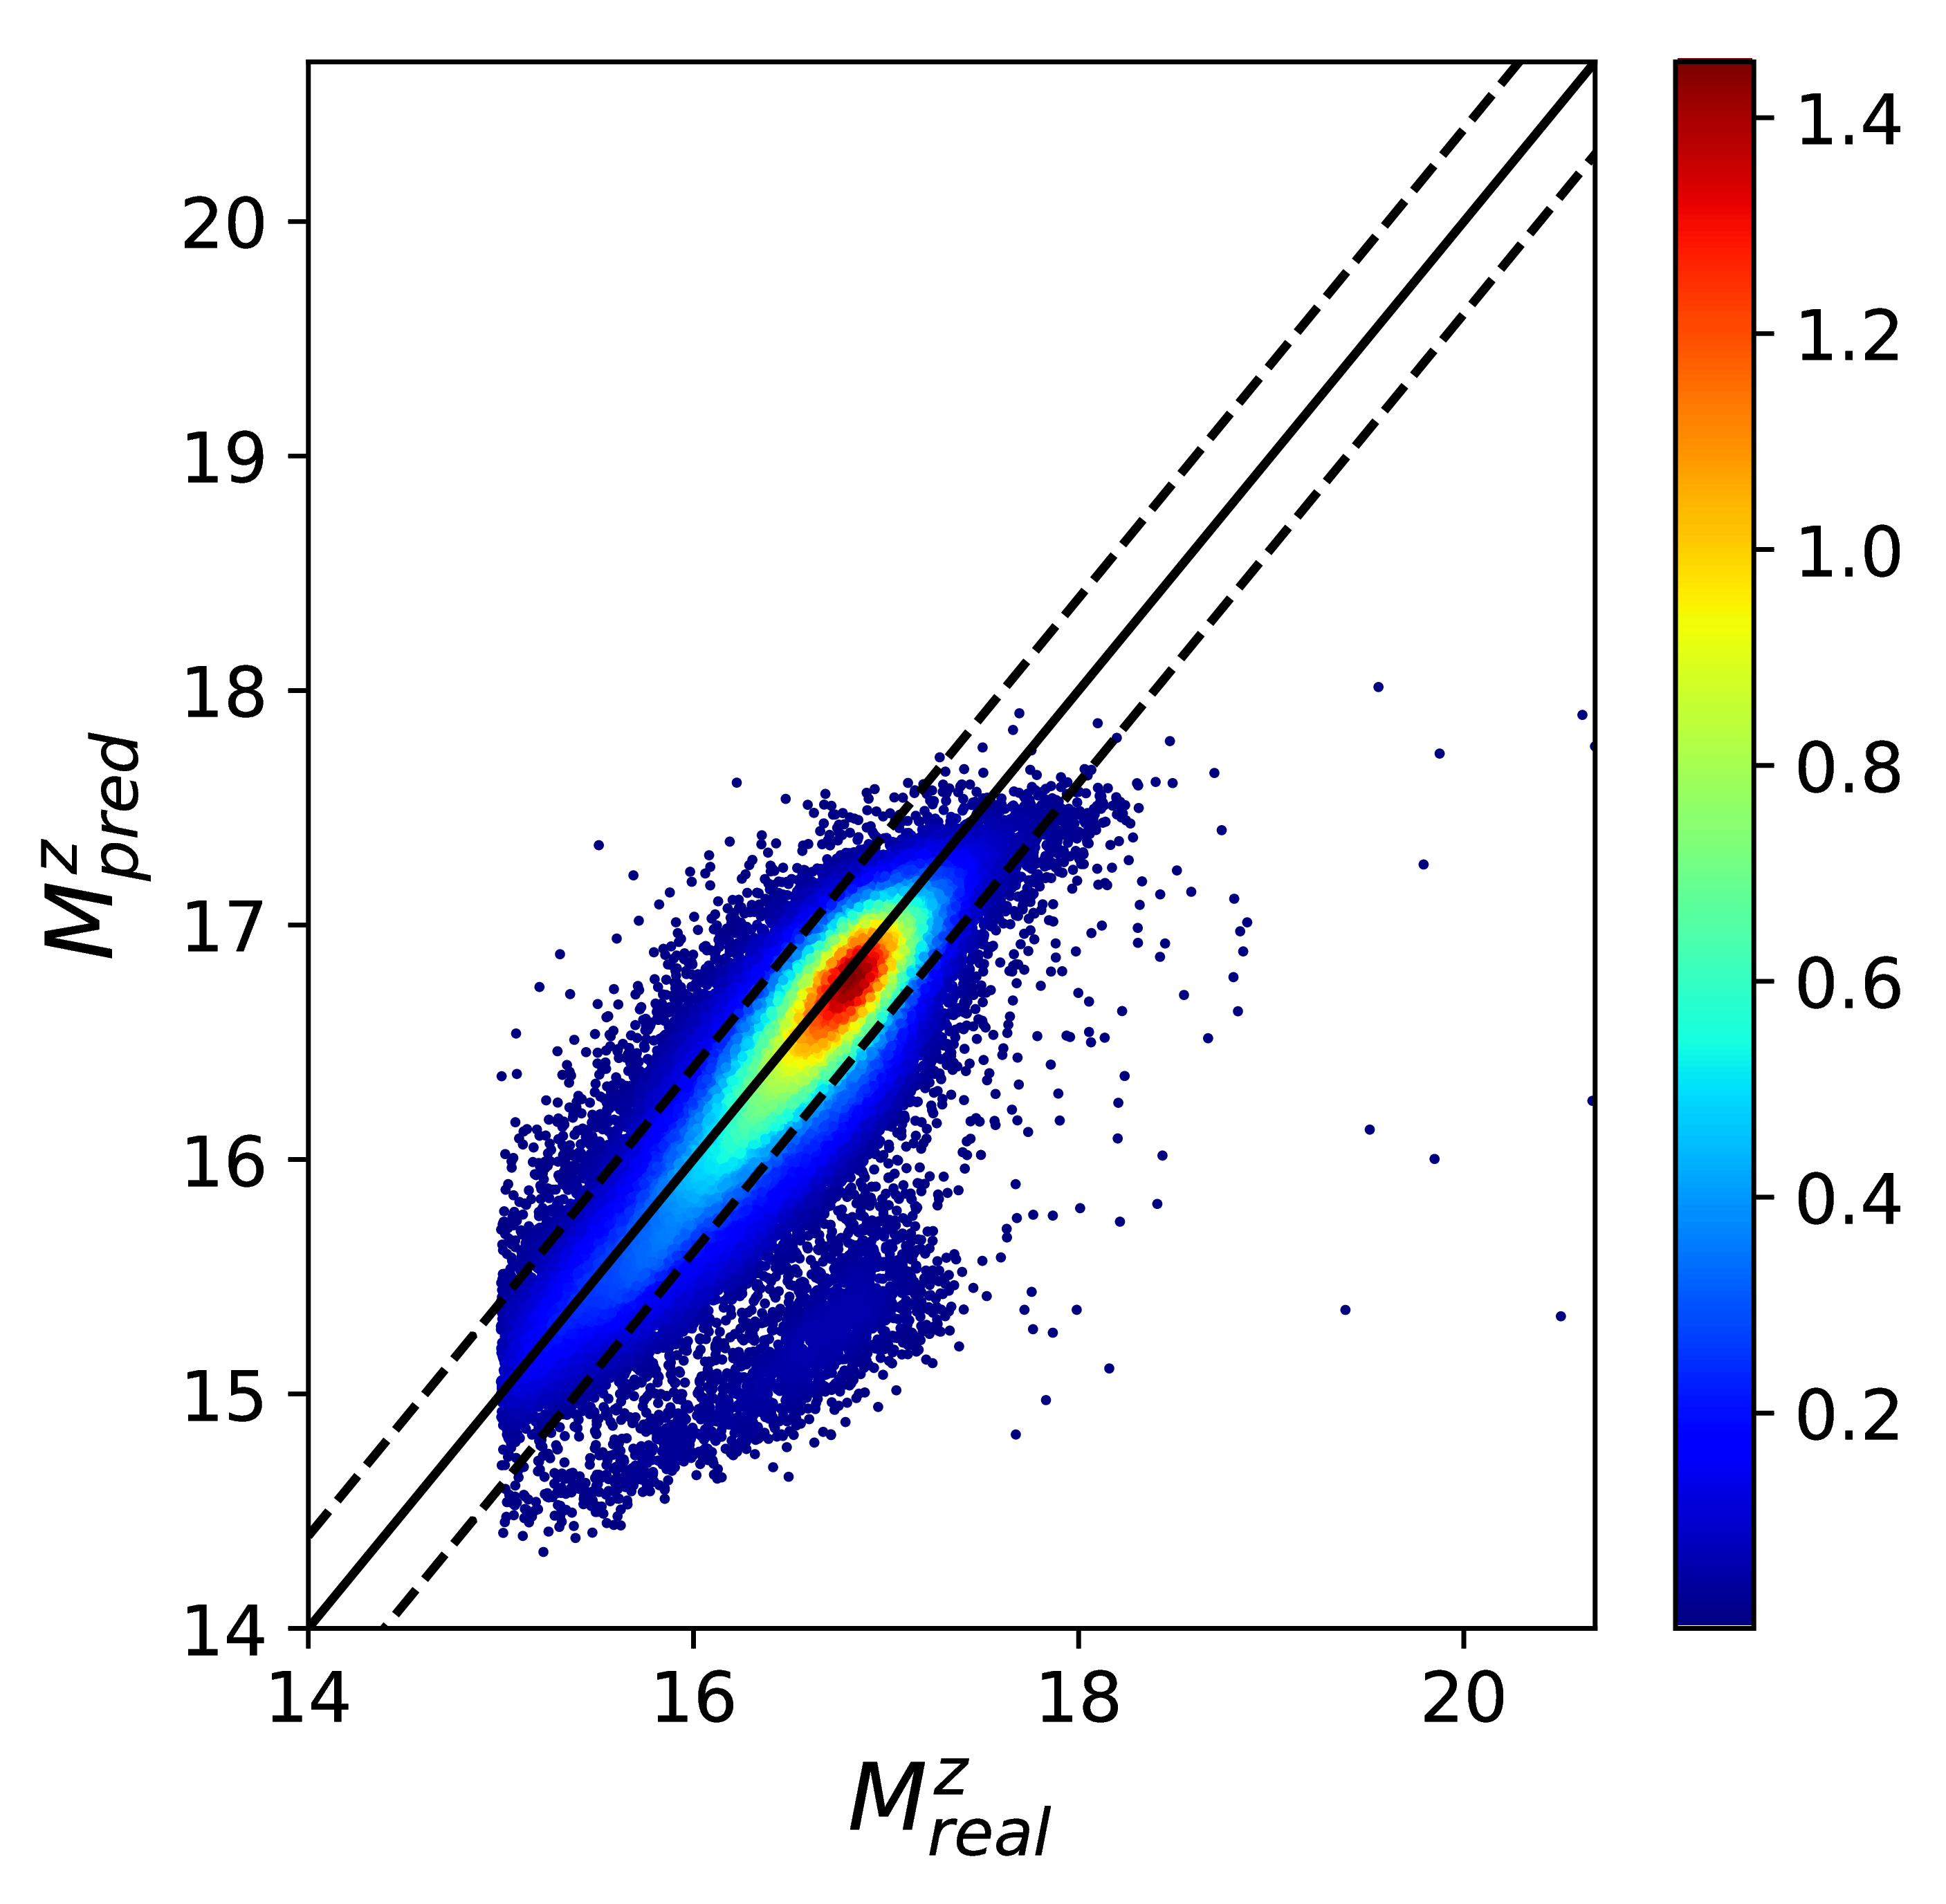
\includegraphics[width=\textwidth, height = \textwidth]{Figures/pmz3.png}
    \label{fig:2}
    
  \end{subfigure}

\caption{Az egyes neurális hálók magniúdópredikciója ábrázolva a valódi magnitúdóértékek függényében.}
\label{mags}
\end{figure}
%%%%%%%%% FIGURES_END %%%%%%%%%%
 Utána a következő konvolúciós réteg $16$ db $2\times 2$-es filterből állt,  \textit{sigmoid} aktivációval, majd egy $2\times 2$-es \textit{MaxPooling} következett. A kijövő értékek kilapítása után következtek a teljesen összekötött rétegek, az első réteg $1024$ neuronból állt, \textit{sigmoid} aktivációval. Utána  $15\%$-os \textit{Dropout} regularizáció következett, ami a túlillesztés elkerülésére szolgált. Ezt követően $512$ neuron, \textit{Relu} aktiváció és $10\%$-os \textit{Dropout}, $256$ neuron \textit{ReLu}-val és végül az egy darab neuron. A hibafüggvény \textit{mean squared error} volt. A \textit{random forest regressor} $250$ fából állt, maximális mélysége $15$, egy levélbe minimum $120$-elemnek kellett kerülnie, egy szétválasztáshoz legalább $28$ minta volt szükséges és a szétválasztás jóságát \textit{mean squared error}-ral mérte. \newline\indent
 A \ref{mags} ábrán látható, hogy az \textit{r} illetve \textit{z} magnitúdókat nagy hibával becsülte, de az adatexploráció felfedte, hogy a \textit{random forest}-nek ezek az adatok kevésbé fontosak. A magnitúdóbecsléseknél az \textit{rmse}-k a következők lettek: $rmse_u = 0.372$, $rmse_g = 0.220$, $rmse_r = 0.397$, $rmse_i = 0.223$, és $rmse_z = 0.393$, az alsó indexek a színt jelölik. 
 \begin{figure}[]
 \centering
  \begin{subfigure}[b]{0.3\textwidth}
    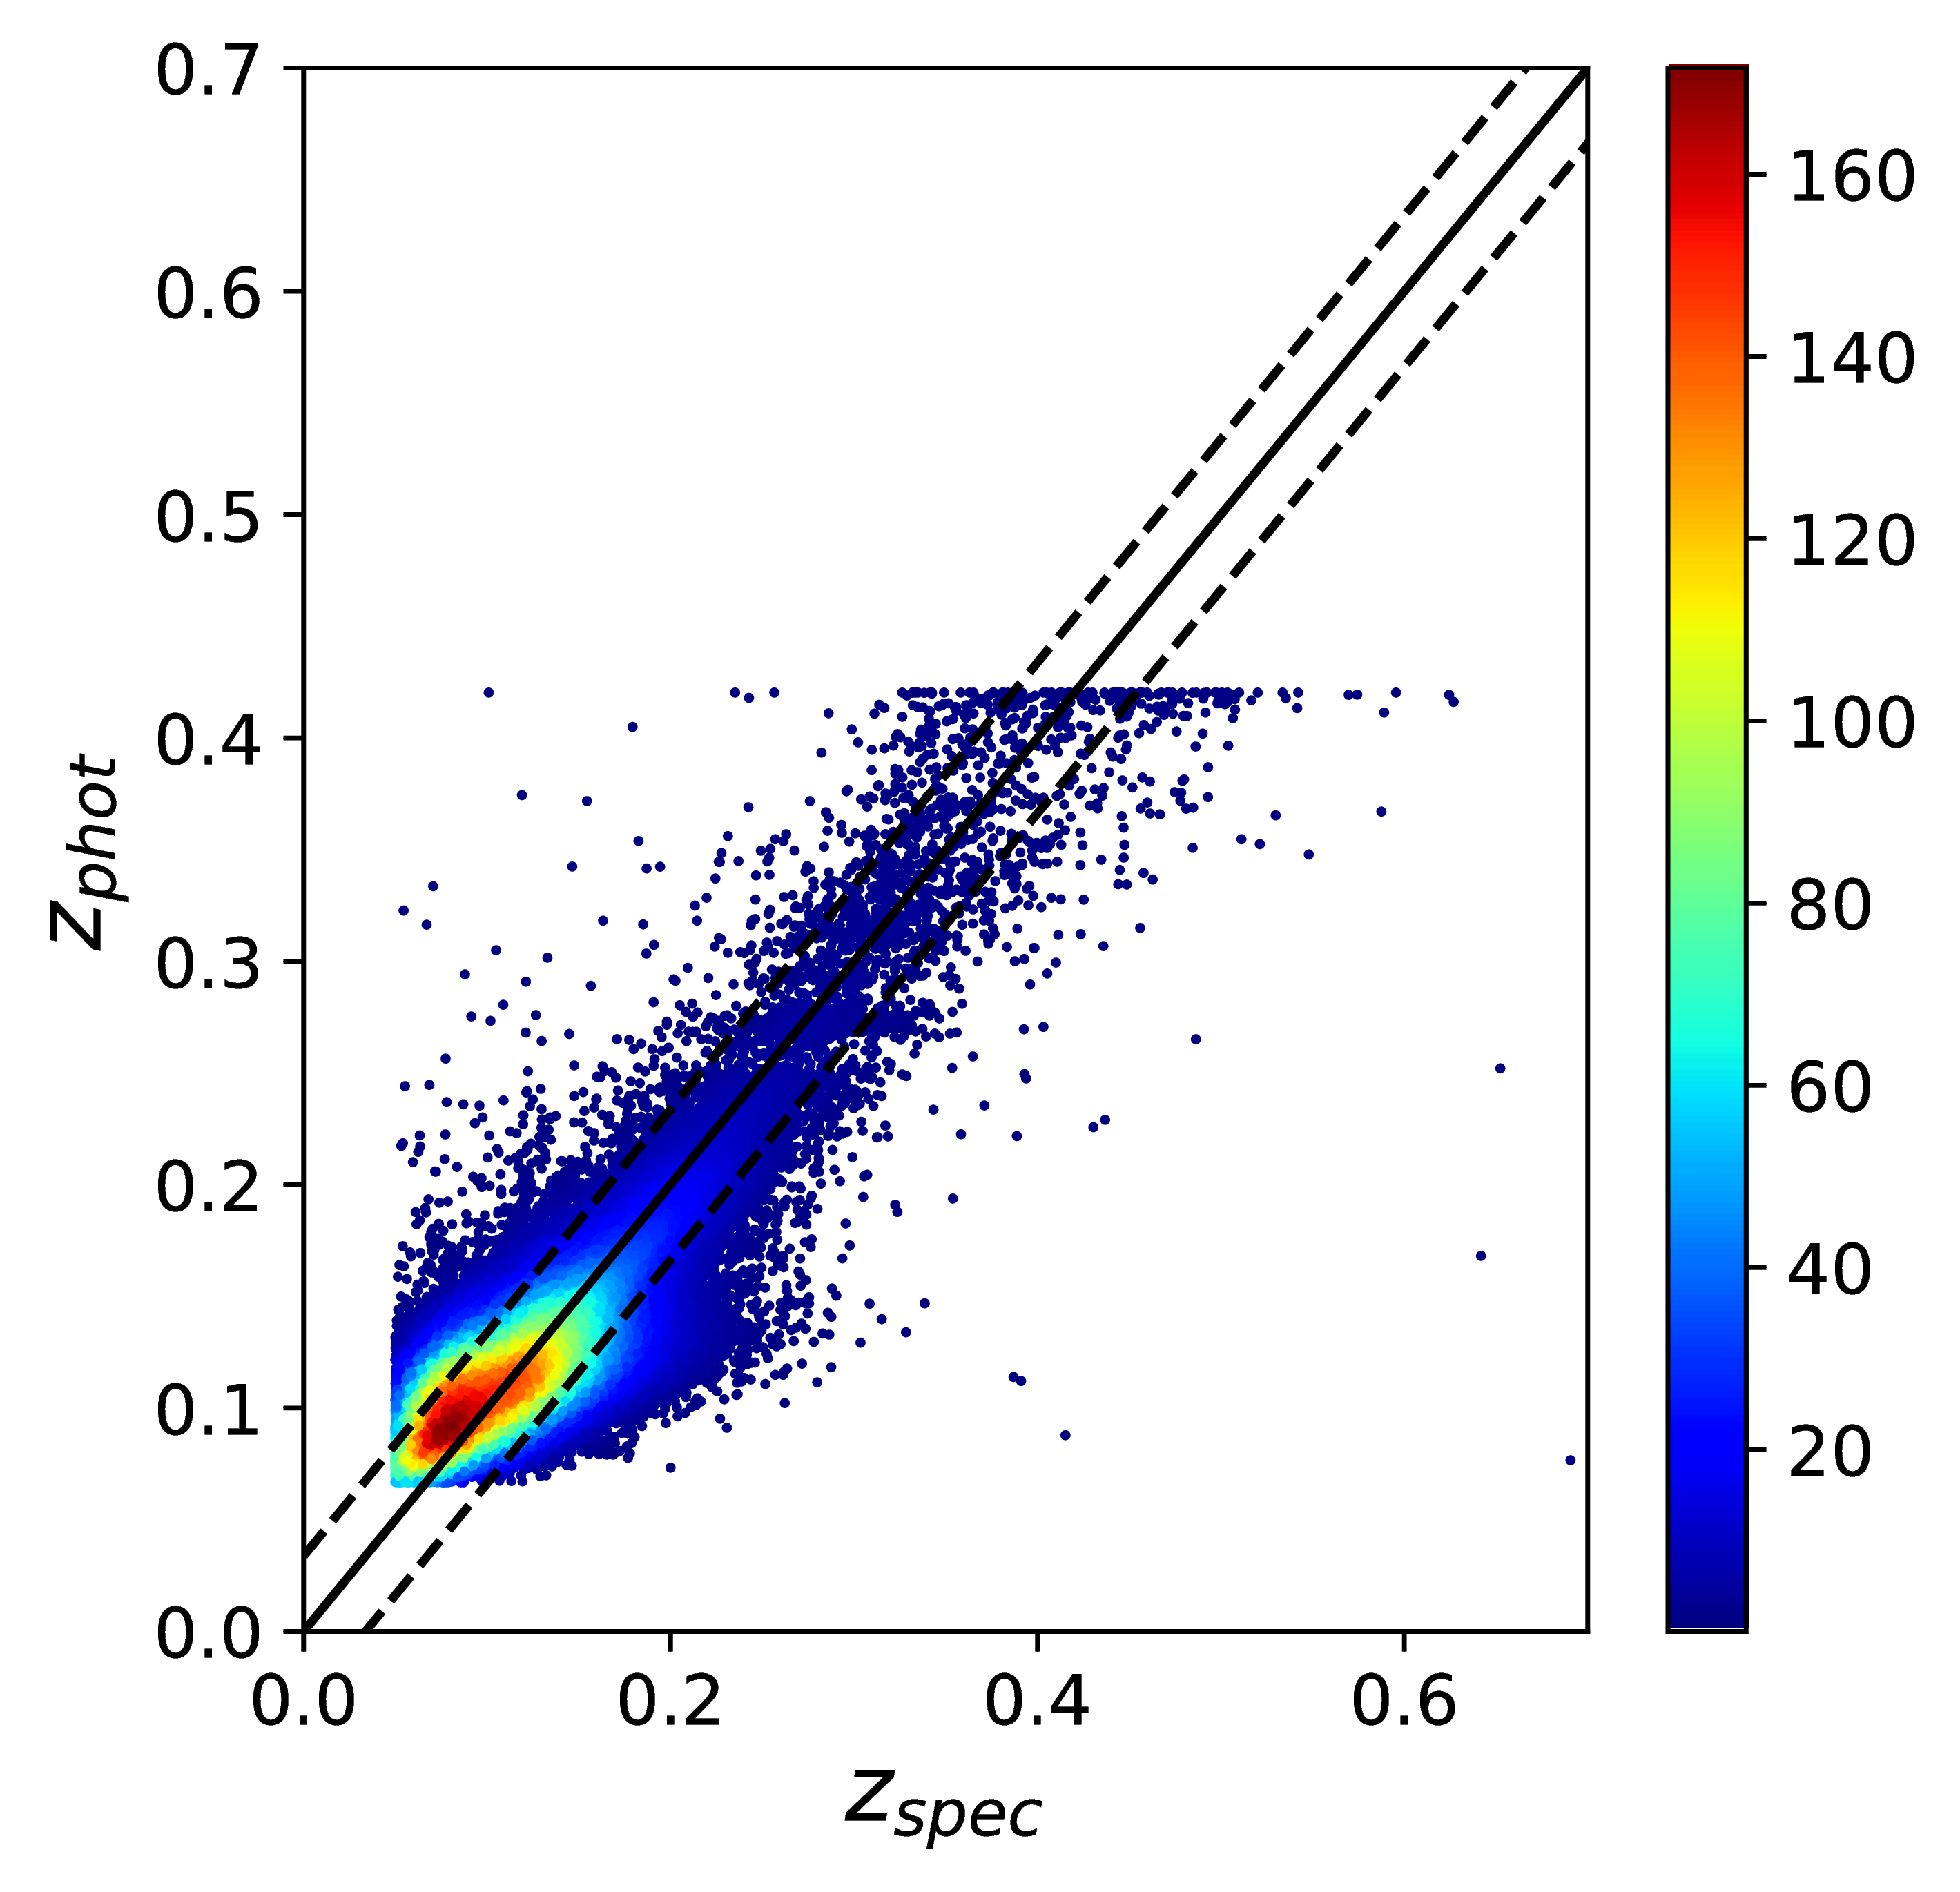
\includegraphics[width=\textwidth, height = \textwidth]{Figures/pRF.png}
    \label{fig:1}
  \end{subfigure}
  \hspace{1.7cm}
  \begin{subfigure}[b]{0.3\textwidth}
    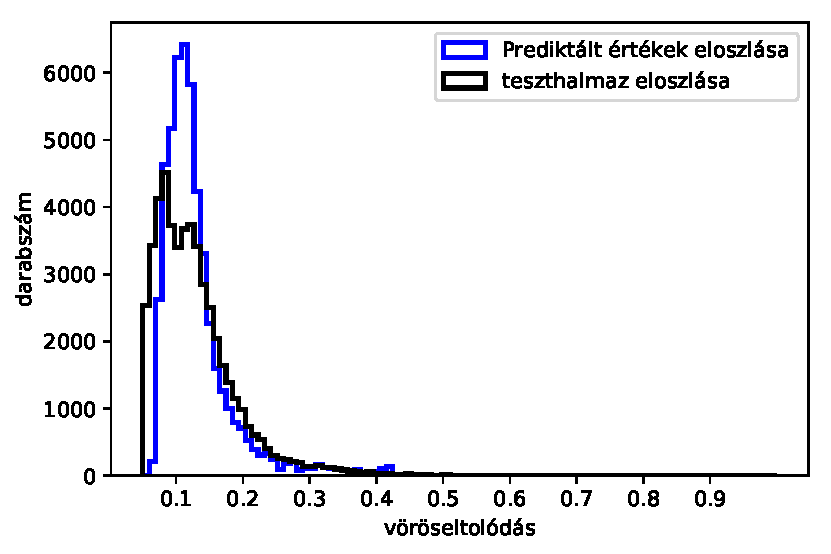
\includegraphics[width=\textwidth, height = \textwidth]{Figures/histrf.pdf}
    \label{fig:2}
  \end{subfigure}
  \caption{A \textit{Random forest} prediktált vöröseltolódás-értékei a spektroszkópiai vöröseltolódások függvényében és a két eloszlás.}
\label{rfp}
\end{figure}
 Ekkora torzítással a magnitúdóadatokon a \textit{random forest} $rmse = 0.0338$ pontossággal tudott becsülni. A becsült és a spektroszkópiai vöröseltolódás-eloszlásokban látszódik a különbség, a prediktált eloszlás görbéje szűkebb, és a csúcs kicsit el van tolódva, ez szisztematikus hiba. A \ref{rfp} bal oldali ábráján látszik, hogy $0.4$-es vöröseltolódás körül vágása van, ez a véletlen erdők extrapolációs képességének hiánya. 
 
 
 \section{Konvolúciós háló kiegészítve becsült magnitúdókkal}
 Neurális hálók tudnak magnitúdókból vöröseltolódást becsülni, de érdekes kipróbálni,hogy hogyan teljesítenek akkor, ha a fényességértékeket csak extra információként kapják meg, a fő adat az ötcsatornás galaxiskép. A magnitúdó adatokat is képekből kell kinyerni, így a \textit{random forest}-nél használt magnitúdó-becslő, tanított hálókat bekötöttem az új háló oldalába, közvetlenül a teljesen összekötött réteg elé. A magnitúdóbecslőket nem tanítottam, hogy ne legyen feleslegesen túl nagy a paraméterszám, ami lassítaná a tanulást. 
 \newline\indent 
 A tanítást az 1-es adathalmaz első $\num{100000}$ képén végeztem, a maradék $\num{50000}$-en a tesztelést, majd megvizsgáltam mire képes a 2-es adathalmaz utolsó $\num{20425}$ galaxisán.
 \begin{figure}[h!]
 \centering
 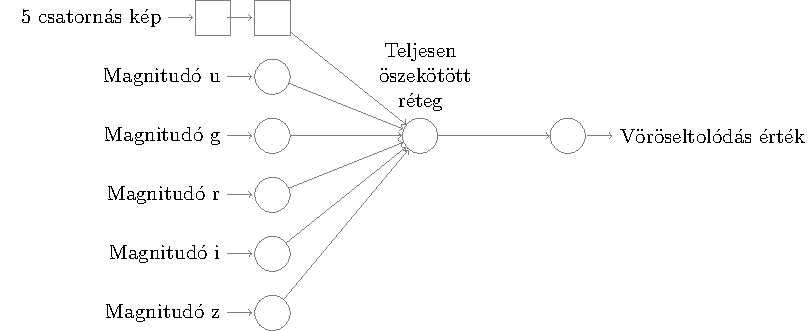
\includegraphics[width = 0.8\textwidth]{Figures/magnet.pdf}
 \caption{A háló sematikus modellje. A magnitúdóbecslő halók kimeneteit és az ötcsatornás képből tanuló konvolúciós rész kimenete közvetlenűl a teljesen összekötött réteg előtt simul egybe.}
 \label{fig:magnet}
 \end{figure}
A 1-es adathalmazon tanult hálót $10$ \textit{epoch} erejéig tanítottam még az 2-es halmazon mielőtt kiértékeltem volna, mert az eltérő tanító-és tesztszett eloszlás problémát jelenthet.\footnote{A felügyelt tanulásnál gyakran alkalmazott az az előfeltételezés, hogy a célváltozó tanító-és teszthalmazának az eloszlása megegyezik. Eltérő esetben, ha tudjuk, hogy a tanuló-és tesztminták nem azonos eloszlásból származnak \textit{covariate shift} módszert lehet alkalmazni a korrigáláshoz \cite{covs}.}
\newline\indent
A haló bementként megkapta az ötcsatornás képet egybe, valamint az öt képet egyesével a magnitúdóbecslő hálóknak. Az első konvolúciós réteg ami az ötcsatornás képen lett alkalmazva

 
 
 \section{Egy mély konvolúciós háló}
 A \textit{random forest}nél láthatóan működött a kinyert adatokból a vöröseltolódás-becslés, de kézenfekvőbb olyan módszert megvalósítani, ami kitalálja, hogy mi a fontos tulajdonság a prediktálás szempontjából, és ezt ki is vonja automatikusan a képből.  
 \newline\indent
 A képi adatokból jól prediktáló konvolúciós hálók\footnote{például VGG16, GoogLeNet} architektúrájához hasonló modellt célszerű készíteni kiindulásként, de ezeket mind osztályozó, objektumfelismerő problémák megoldására használták, tanítására több adat és számítási kapacitás állt rendelkezésre, ezért a vöröseltolódás-becslő háló nem lesz olyan \textit{mély}. A háló tanítását a 2-es adathalmaz első $\num{80000}$ képével végeztem, majd a maradék $\num{20425}$ képpel teszteltem. Valamint végeztem tesztelést az összehasonlítás édekében az 1-es adathalmaz $\num{100000}$-től $1500000$-ig elhelyezekdő képeivel is.\newline\indent A modell architektúrája a következő volt: a bemenet az $50\times50\times5$ méretű kép volt, utána kétszer egymás után, 48 darab $3\times 3$-as \textit{filter}ekből álló konvolúciós réteg, majd $2\times 2$ \textit{Averagepooling}. Utána következett 3 egymás utáni $96$ $3\times3$ \textit{filter}ből álló réteg, majd megint egy $2\times2$-es \textit{Averagepooling}, majd kétszer $200$ darab $3\times3$ \textit{filter}, $2\times 2$ \textit{Averagepooling}, egy $200$ \textit{filter}es, $3\times 3$ konvolúciós réteg, egy \textit{BatchNormalizáció}, majd megint egy $200$ darab, $3\times 3$-as \textit{filter}es réteg. Aztán $2\times 2$-es \textit{Averagepooling}, majd egy $200$ és egy $20$ darabos $3\times 3$ \textit{filter}es réteg, utána $72$ darab $1\times 1$ \textit{filteres} dimenzió csökkentő konvolúciós réteg.
\begin{figure}[h!]
 \centering
  \begin{subfigure}[b]{0.3\textwidth}
    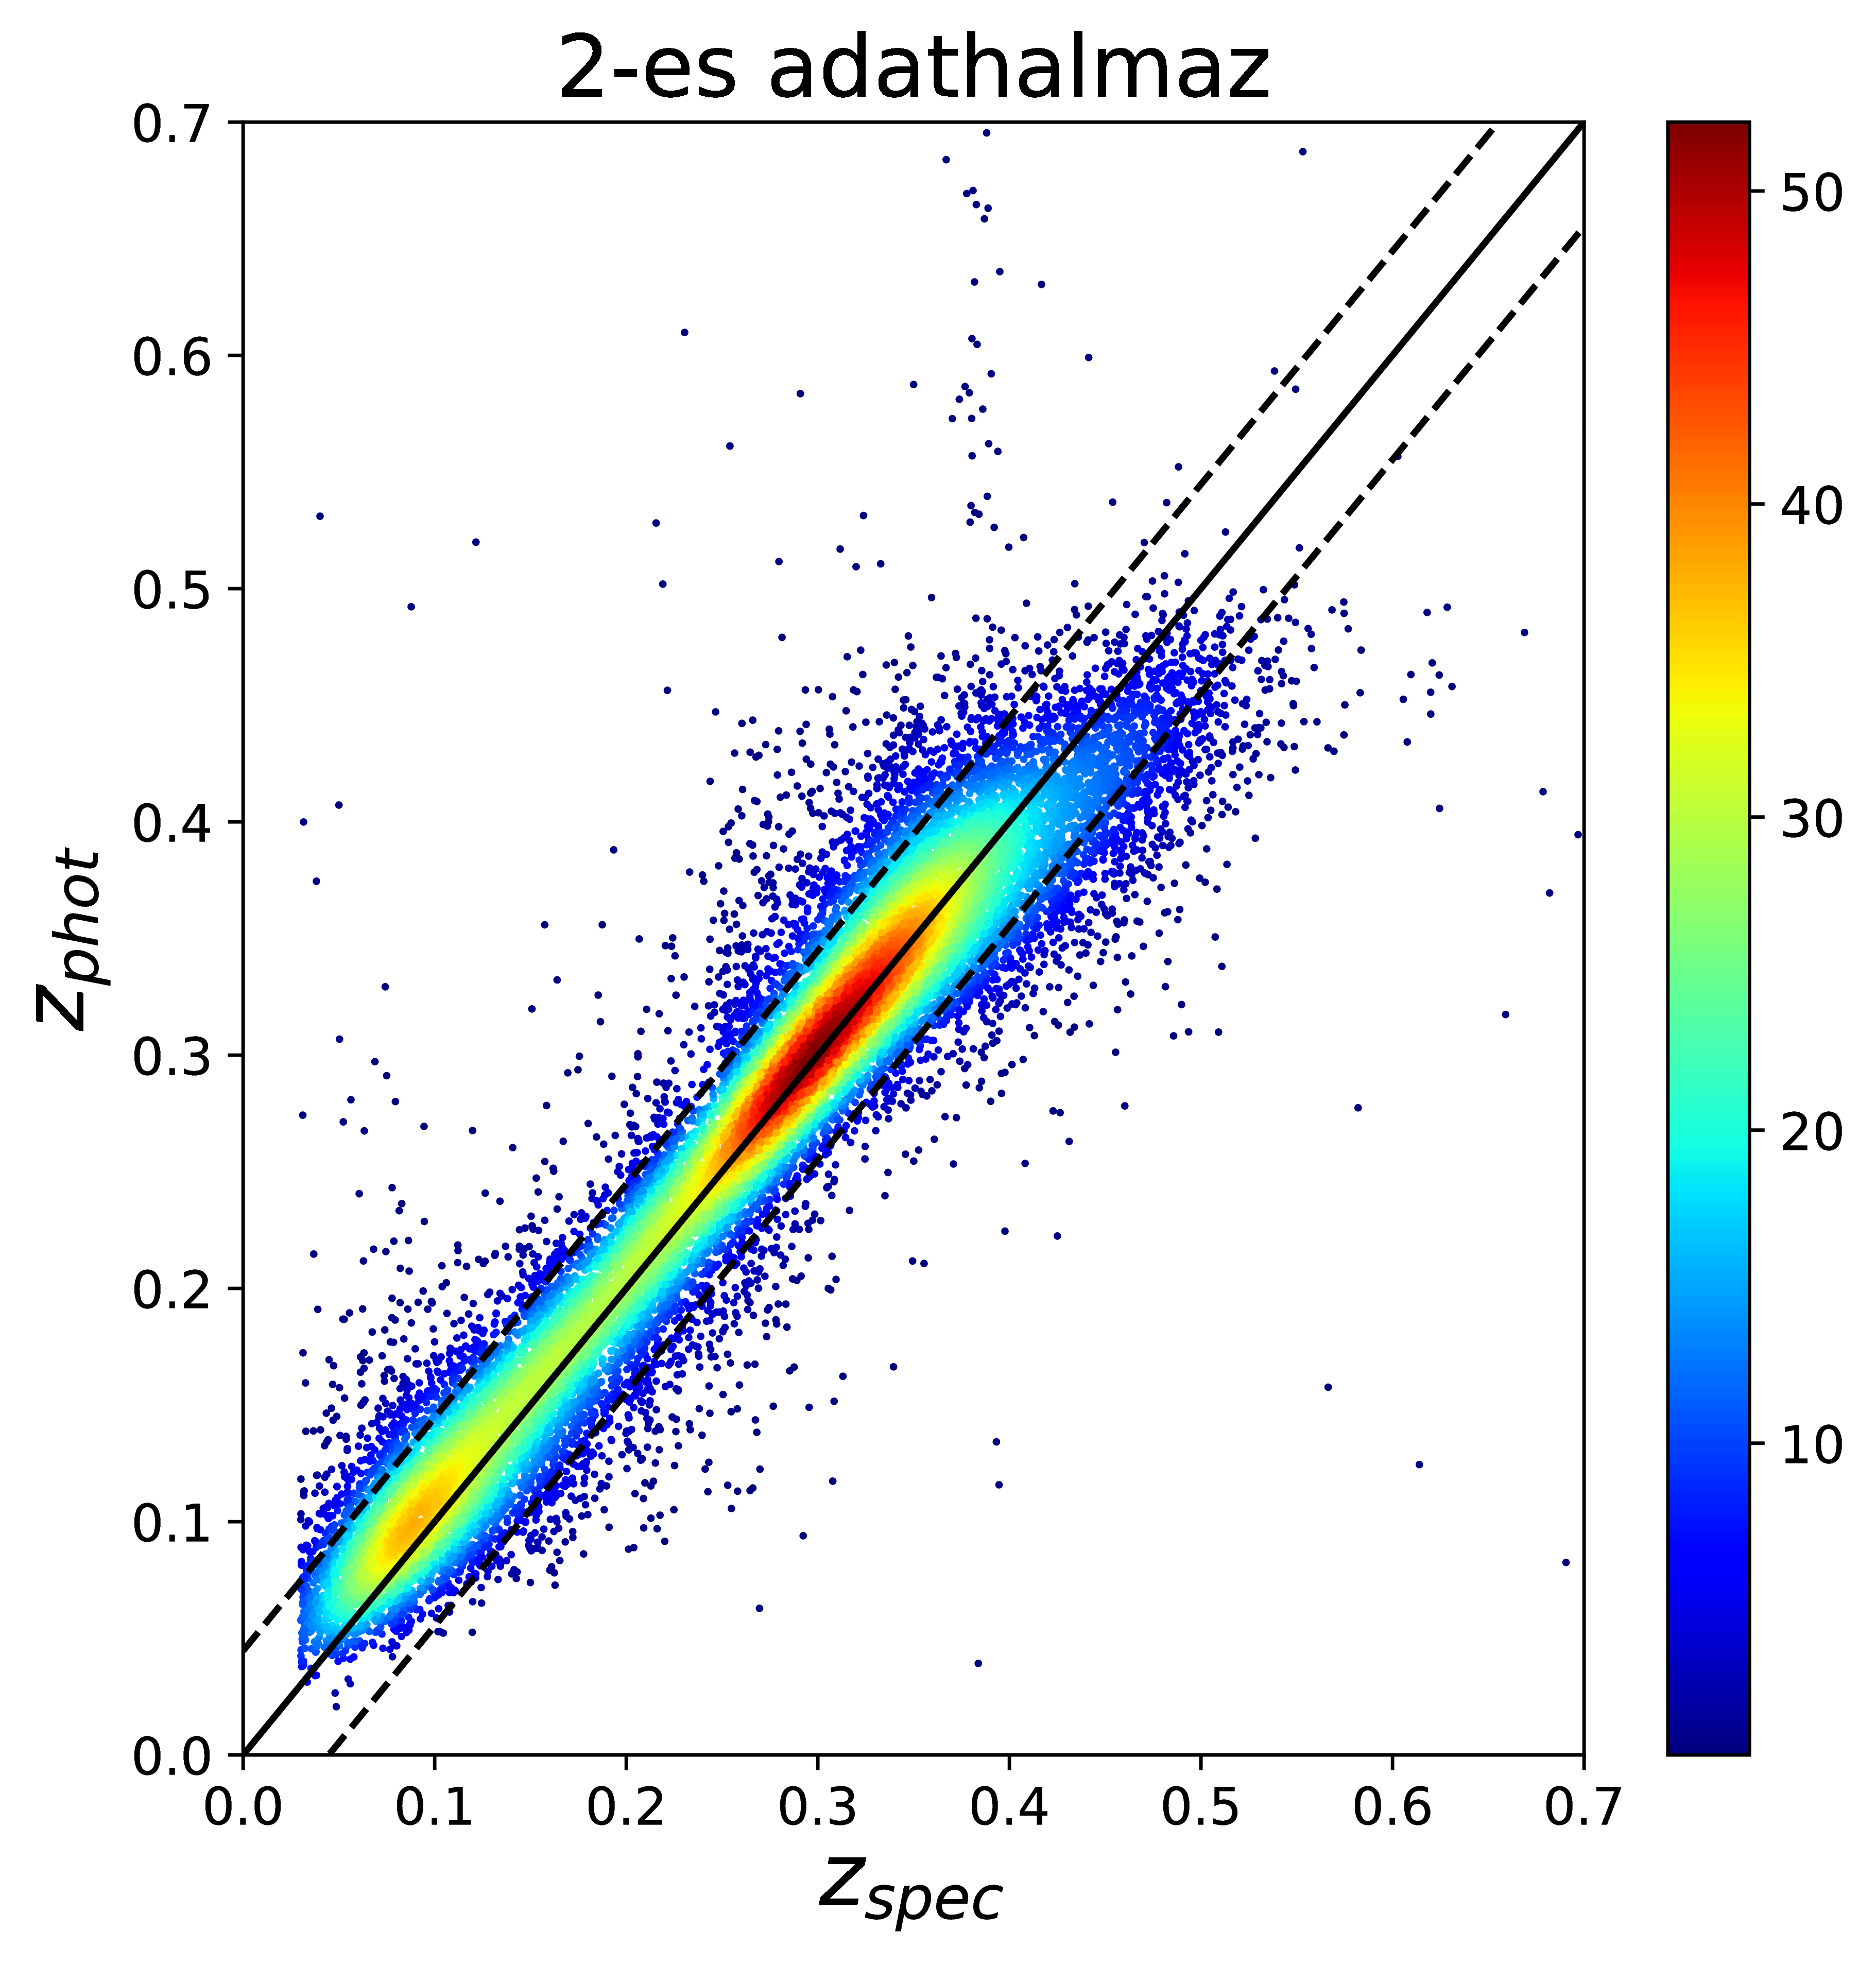
\includegraphics[width=\textwidth, height = \textwidth]{Figures/plotCNN2.png}
    \label{fig:1}
  \end{subfigure}
  \hspace{1.7cm}
  \begin{subfigure}[b]{0.3\textwidth}
    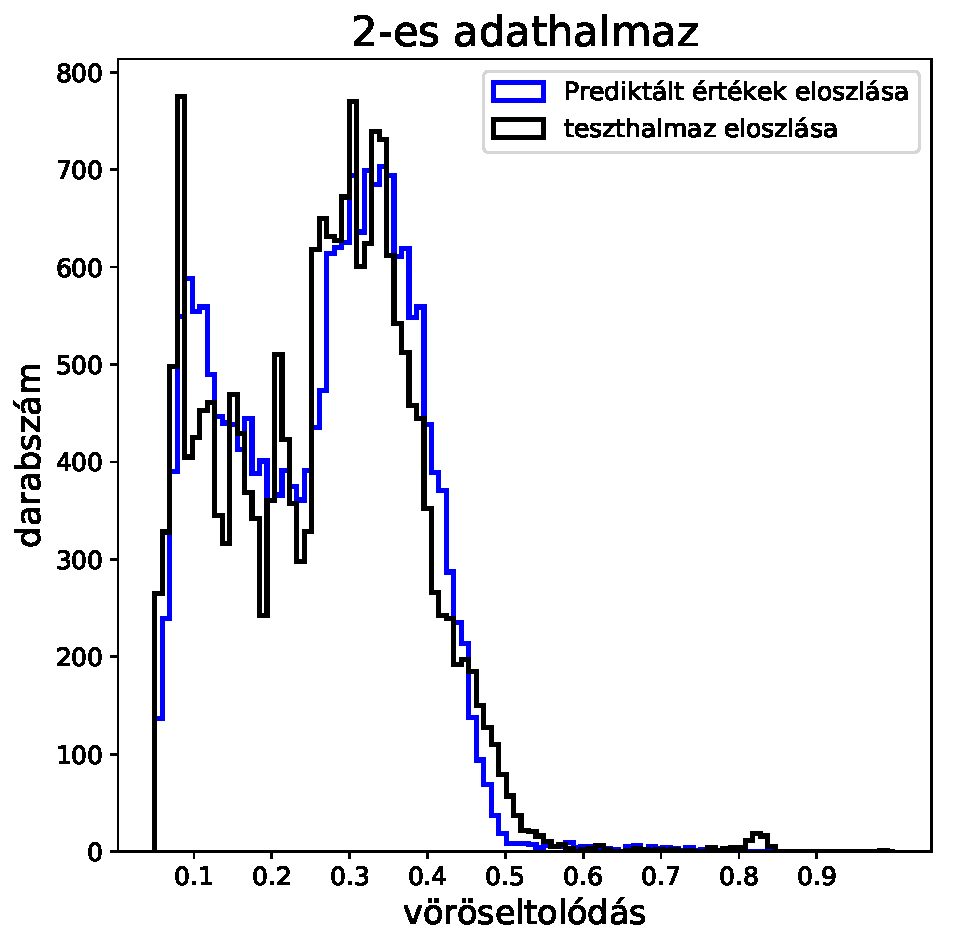
\includegraphics[width=\textwidth, height = \textwidth]{Figures/histCNN2.pdf}
    \label{fig:2}
  \end{subfigure}
  \caption{A konvolúciós neurális háló becslései a spektroszkópiai vöröseltolódás-értékek függvényében a 2-es adathalmazon, és a vöröseltolódás-eloszlások.}
\label{cnn}
\end{figure}
Mindegyik rétegen \textit{ReLU} aktivációt alkalmaztam. A teljesen összekötött rész $\num{4096}$ neuronnal kezdődőtt, majd $400$ neuron a következő rétegben, mind \textit{ReLU} aktivációval, végül az $1$ neuronból álló kimeneti réteg, aktiváció nélkül.
 \newline \indent
A tanításhoz a megnövekedett paraméterszám miatt több \textit{epoch}ra volt szükség, mint a magnitúdóbecslésnél, összesen $100$ \textit{epoch}-ra, a \textit{learning rate}-et  csökkentettem, ha nem csökkent a hiba értéke, illetve a \textit{batch size}-t növeltem. A 2-es adathalmazon a $\num{20425}$ galaxison tesztelve a $\textit{rmse} = 0.0447$ lett. A \ref{cnn} ábra bal oldalán látható, hogy a prediktált értékeket jelölő pontok szimmetrikusak a $45^{\circ}$-os egyenesre a $0.2$ és $0.45$ közötti vöröseltolódás-tartományon, nincsen szisztematikus hibája. A $0.2$-nél kisebb vöröseltolódásokat gyengén felülbecsli, a $0.5$-nél nagyobb vöröseltolódásúakat pedig alul. Érdemes volt megnézni, hogyan teljesít a háló az 1-es adathalmazon, ahol több alacsony vöröseltolódású galaxist tartalmaz a tesztszett, valamint így összehasonlítható a \textit{random forest} módszerrel. Mielőtt prediktáltattam volna a modellt, tanítottam $10$ \textit{epoch}-ot az 1-es adathalmazon.

\begin{figure}[]
 \centering
  \begin{subfigure}[b]{0.3\textwidth}
    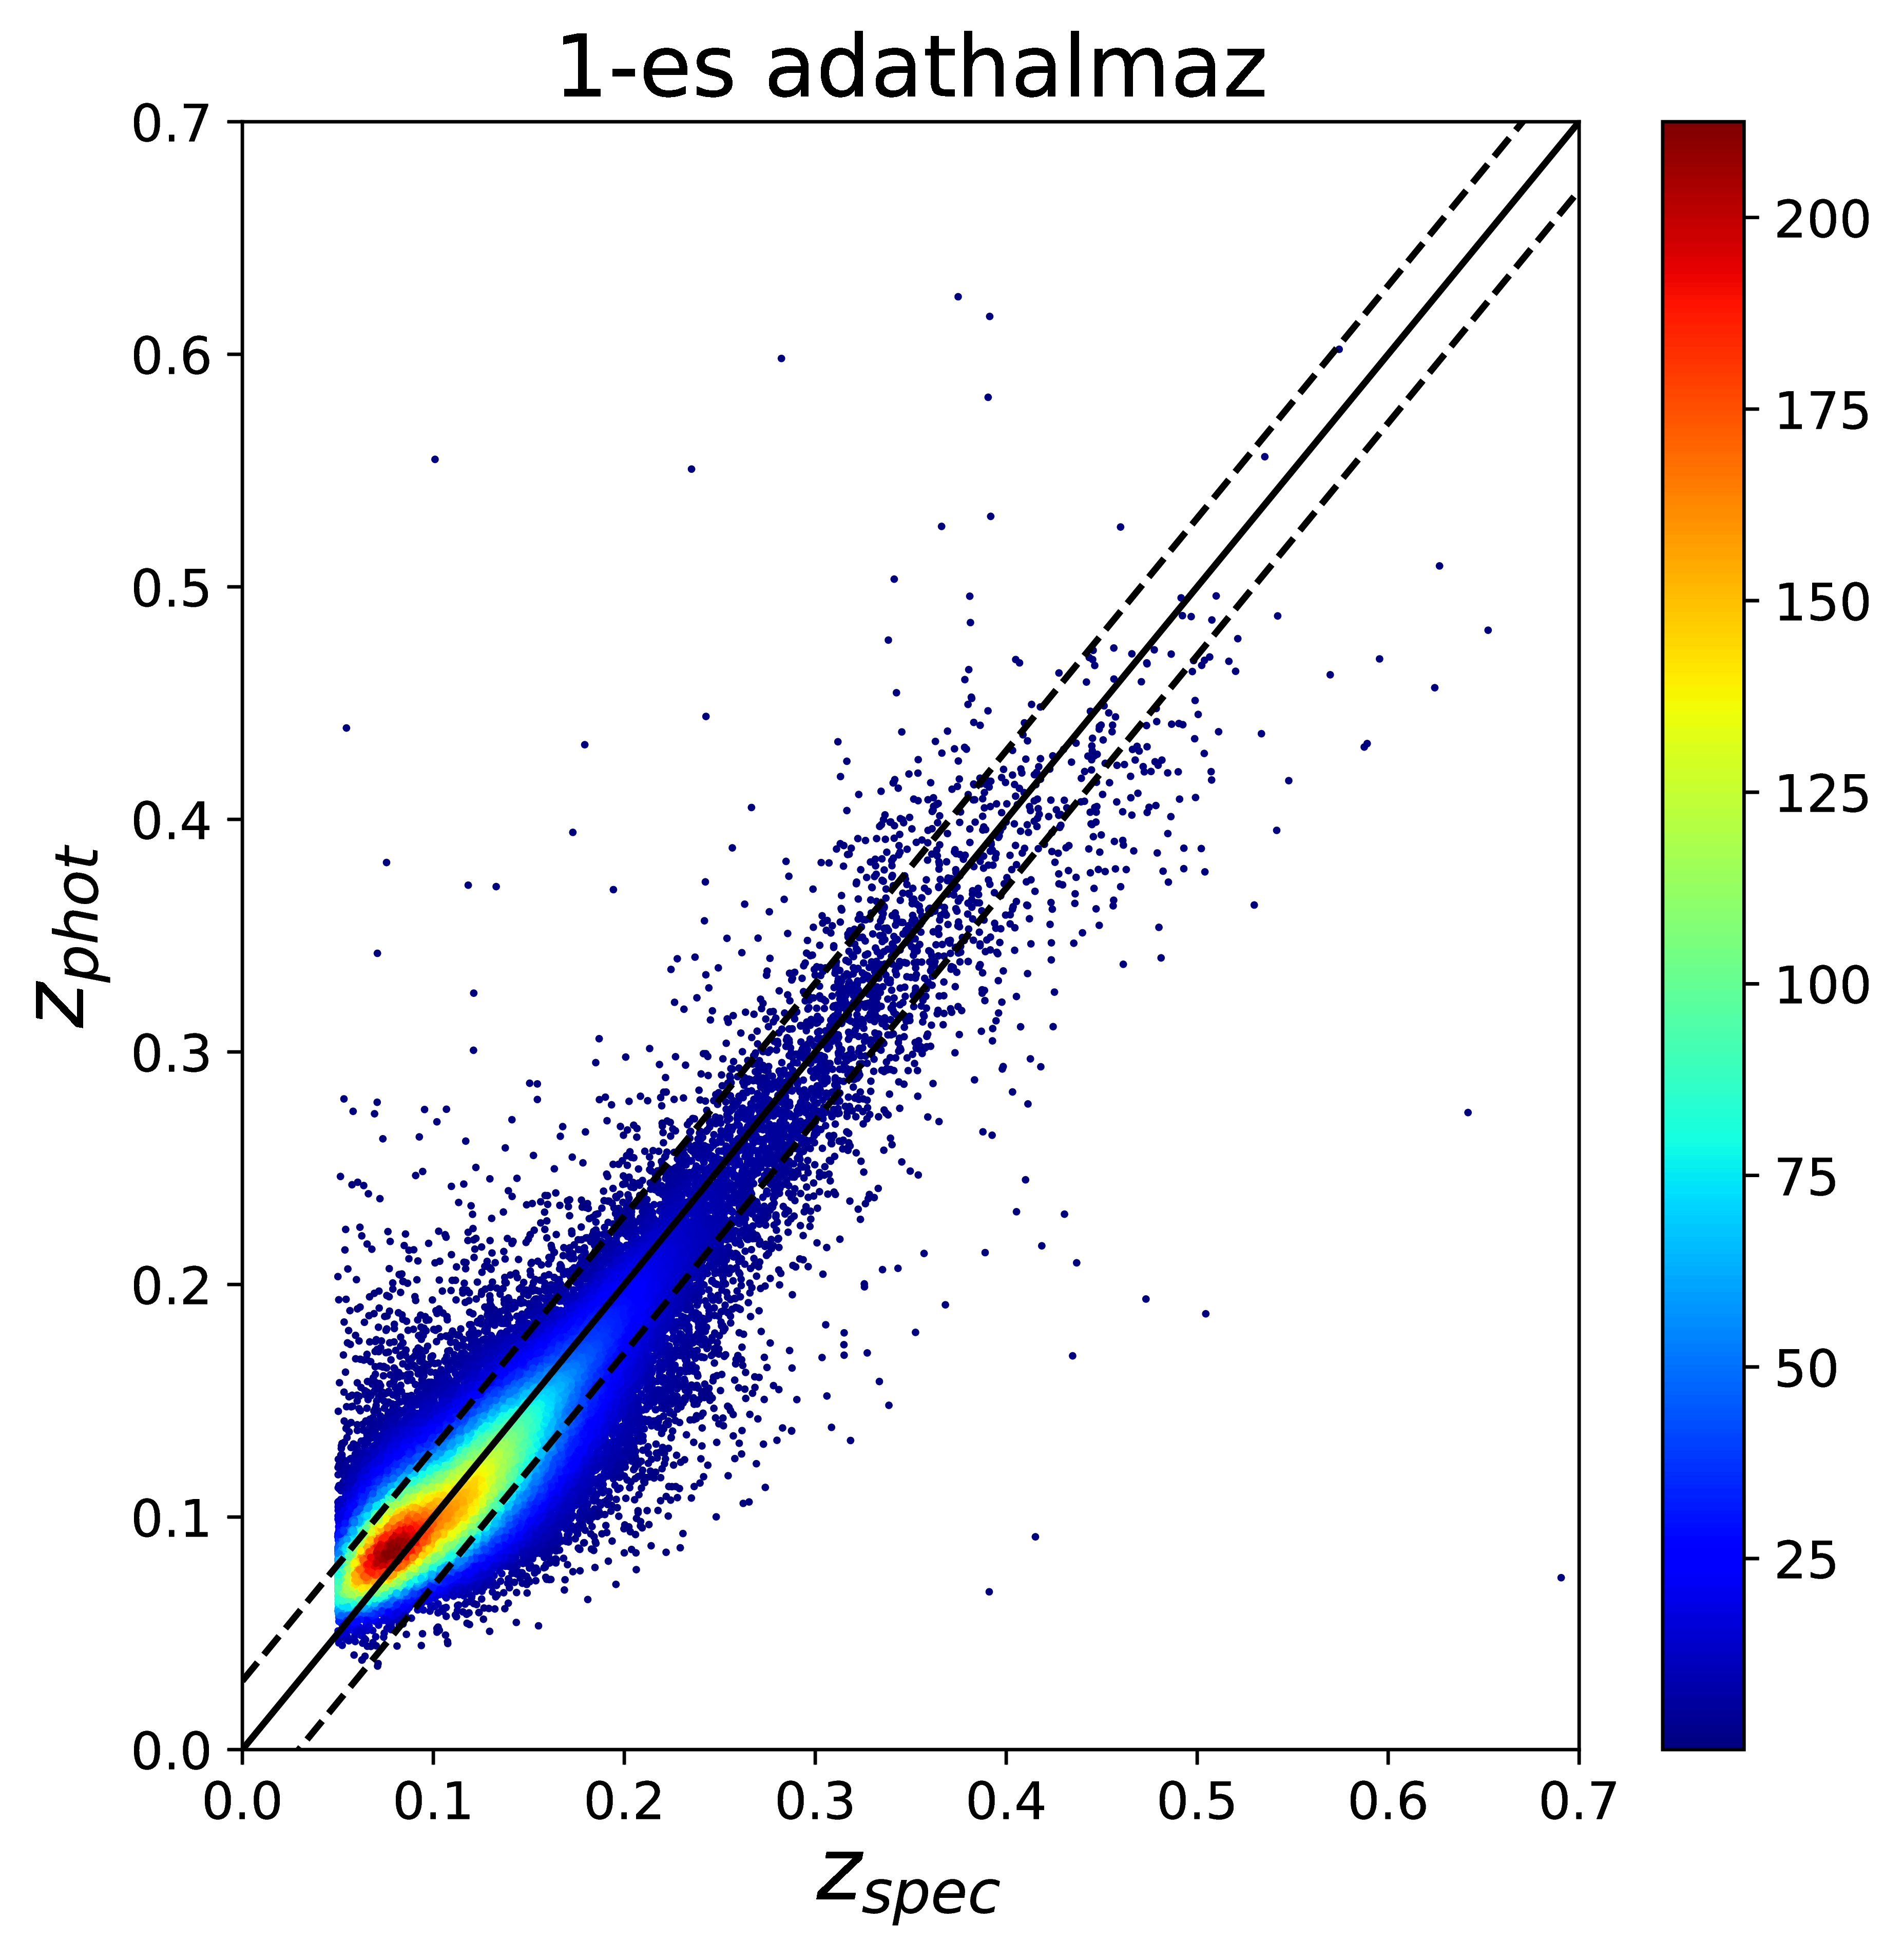
\includegraphics[width=\textwidth, height = \textwidth]{Figures/plotCNN1.png}
    \label{fig:1}
  \end{subfigure}
  \hspace{1.7cm}
  \begin{subfigure}[b]{0.3\textwidth}
    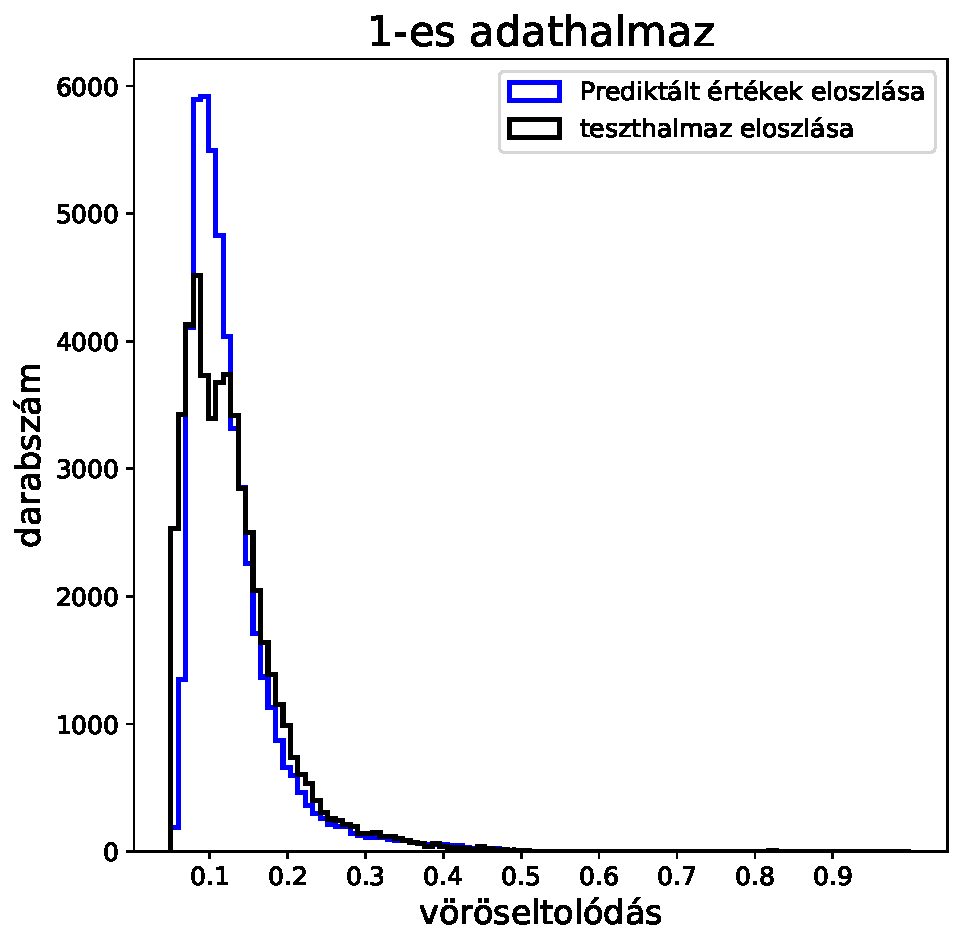
\includegraphics[width=\textwidth, height = \textwidth]{Figures/histCNN1.pdf}
    \label{fig:2}
  \end{subfigure}
  \caption{A konvolúciós neurális háló becslései a spektroszkópiai vöröseltolódás-értékek függvényében a 1-es adathalmazon, és a vöröseltolódás-eloszlások.}
\label{cnn1}
\end{figure}

A tesztadatokon $\textit{rmse} =0.0295$ hibát produkált, ami jobb mint a \textit{random forest}é, viszont az alacsony vöröseltolódásoknál még mindig enyhén felülbecsül. Megjegyezendő, hogy az 2-es tanítóhalmaz és az 1-es teszthalmaz $2.6\%$-ban átfed, ez okozhat \textit{rmse} csökkenést, de nem nagy mértékben, a tanítóhalmazban a modell által már látott galaxisok vöröseltolódás-becslésének hibáját $0$-nak véve, a csak teszthalmazban megkapott mintákon a $rmse = 0.0298$.
\newline\indent
Ez a módszer jól alakalmazható a feltételezéssel...


  \chapter{Összegzés}
\newpage













\begin{thebibliography}{99\kern\bibindent}
\def\bibindent{1em}

\makeatletter
\let\old@biblabel\@biblabel
\def\@biblabel#1{\old@biblabel{#1}\kern\bibindent}
\let\old@bibitem\bibitem
\def\bibitem#1{\old@bibitem{#1}\leavevmode\kern-\bibindent}
\makeatother
\addcontentsline{toc}{chapter}{Irodalomjegyzék}
\bibitem{fr}Z. Frei and A. Patkós, Inflációs Kozmológia: (Typotex, Budapest, 2005).



%%%2    %%%%%   photo z
\bibitem{baum} Baum, W. A.: 1962, Problems of Extra-Galactic Research, Proceedings from IAU Symposium no. 15. Edited by George Cunliffe McVittie. International Astronomical Union Symposium no. 15, Macmillan Press, New York, p.390


\bibitem{webp}“Photometric Redshifts.” NASA/IPAC Extragalactic Database - NED, ned.ipac.caltech.edu/level5/Glossary/Essay\_{}photredshifts.html.


\bibitem{Koo}Koo, D. C. “Optical Multicolors - A Poor Person's Z Machine for Galaxies.” The Astronomical Journal, vol. 90, 1985, p. 418., doi:10.1086/113748.

\bibitem{bruzual}Bruzual, G., and S. Charlot. “Stellar Population Synthesis at the Resolution of 2003.” Monthly Notices of the Royal Astronomical Society, vol. 344, no. 4, 2003, pp. 1000–1028., doi:10.1046/j.1365-8711.2003.06897.x.


\bibitem{hild}Hildebrandt, H., et al. “PHAT: PHoto-ZAccuracy Testing.” Astronomy \&{} Astrophysics, vol. 523, 2010, doi:10.1051/0004-6361/201014885.



\bibitem{connoly et al}Connolly, A. J., et al. “Slicing Through Multicolor Space: Galaxy Redshifts from Broadband Photometry.” The Astronomical Journal, vol. 110, 1995, p. 2655., doi:10.1086/117720.

\bibitem{app_photoz} Csabai, I., et al. “The Application of Photometric Redshifts to the SDSS Early Data Release.” The Astronomical Journal, vol. 125, no. 2, 2003, pp. 580–592., doi:10.1086/345883.

\bibitem{rf}Carliles, S., et al. “Random Forests For Photometric Redshifts.” The Astrophysical Journal, vol. 712, no. 1, 2010, pp. 511–515., doi:10.1088/0004-637x/712/1/511.

%%     2      %% ML
\bibitem{mlrsone}Collister, Adrian A., and Ofer Lahav. “ANNz: Estimating Photometric Redshifts Using Artificial Neural Networks.” Publications of the Astronomical Society of the Pacific, vol. 116, no. 818, 2004, pp. 345–351., doi:10.1086/383254.

\bibitem{mlrstwo}Csabai, I., et al. “Multidimensional Indexing Tools for the Virtual Observatory.” Astronomische Nachrichten, vol. 328, no. 8, 2007, pp. 852–857., doi:10.1002/asna.200710817.

\bibitem{mlrstwo}Collister, Adrian A., and Ofer Lahav. “ANNz: Estimating Photometric Redshifts Using Artificial Neural Networks.” Publications of the Astronomical Society of the Pacific, vol. 116, no. 818, 2004, pp. 345–351., doi:10.1086/383254.

\bibitem{randomF}Ball, Nicholas M., and Robert J. Brunner. “Data Mining And Machine Learning In Astronomy.” International Journal of Modern Physics D, vol. 19, no. 07, 2010, pp. 1049–1106., doi:10.1142/s0218271810017160.

\bibitem{rf2}“Random Forests Leo Breiman and Adele Cutler.” Statistics at UC Berkeley, www.stat.berkeley.edu/~breiman/RandomForests/.


\bibitem{mlrsthree}Sadeh, I., et al. “ANNz2: Photometric Redshift and Probability Distribution Function Estimation Using Machine Learning.” Publications of the Astronomical Society of the Pacific, vol. 128, no. 968, 2016, p. 104502., doi:10.1088/1538-3873/128/968/104502.

\bibitem{batchs}L., Samuel, et al. “Don't Decay the Learning Rate, Increase the Batch Size.” SAO/NASA ADS: ADS Home Page, 1 Nov. 2017, adsabs.harvard.edu/cgi-bin/bib\_{}query?arXiv\%{}3A1711.00489.
%%%     3 %%%%% SDSS
\bibitem{sdssV}Zasowski, Gail. Science Blog from the SDSS, blog.sdss.org/2018/02/21/sdss-v-is-underway/.

%%%% 3 %%%% Trainset
\bibitem{sci}“SciServer – Collaborative Data-Driven Science.” SciServer, www.sciserver.org/.

\bibitem{rsd}Verevkin, A. O., et al. “The Non-Uniform Distribution of Galaxies from Data of the SDSS DR7 Survey.” Astronomy Reports, vol. 55, no. 4, 2011, pp. 324–340., doi:10.1134/s1063772911020089.

\bibitem{covs}Mcgaughey, Georgia, et al. “Understanding Covariate Shift in Model Performance.” F1000Research, vol. 5, 2016, p. 597., doi:10.12688/f1000research.8317.3.

\end{thebibliography}





\chapter*{Nyilatkozat}

\noindent
\textbf{Név:} Horváth Bendegúz
\\
\textbf{ELTE Természettudományi Kar, szak:} Fizika BSc
\\
\textbf{Neptun azonosító:} ZNL3LK\\
\textbf{Szakdolgozat címe:} Fotometrikus vöröseltolódás becslés
\vspace*{2cm}    

A    \textbf{szakdolgozat}   szerzőjeként    fegyelmi
felelősségem  tudatában kijelentem,  hogy a  dolgozatom  önálló munkám
eredménye, saját  szellemi termékem, abban a  hivatkozások és idézések
standard  szabályait  következetesen   alkalmaztam,  mások  által  írt
részeket a megfelelő idézés nélkül nem használtam fel.

\vspace*{2cm}
Budapest 2018. majus ?.
\\
\hspace*{8 cm}\rule{5cm}{0.5pt}
\end{document}

